%!TEX root = /Users/stevenmartell/Documents/CURRENT PROJECTS/iSCAM-trunk/fba/BC-herring-2011/WRITEUP/BCHerring2011.tex
\section{Results}
The results section is broken down into three major subsections, Maximum likelihood fits to the data, marginal posterior distributions, and stock forecasts and catch advice based on samples from the joint posterior distribution.

\subsection{Maximum likelihood fits to the data}
Although  the maximum likelihood estimates are not explicitly used for constructing the catch advice, we do present the MLE estimates of the residual patterns and fits to the data for comparisons.

\subsubsection{Catch residuals}
Residuals between the observed and predicted catch are largely determined by the user specified standard deviation in each of the control files.  In this assessment, the assumed variance for all regions (including minor regions) was set at 0.005, which corresponds to a standard deviation of approximately 0.0707.  Overall the residuals for each fishery in each stock assessment region are unremarkable (Fig. \ref{PartII:Results:fig1}), with exception of a  major outlier in the Haida Gwaii in the mide 1950s.  In 1956, the reported catch in Haida Gwaii was extremely large ($>$ 60,000 mt) and the model has a difficult time explaining this large catch. In order to explain this large catch in a single year, a large biomass in the region is required.

\begin{figure}[!tbp]
	% Requires \usepackage{graphicx}
	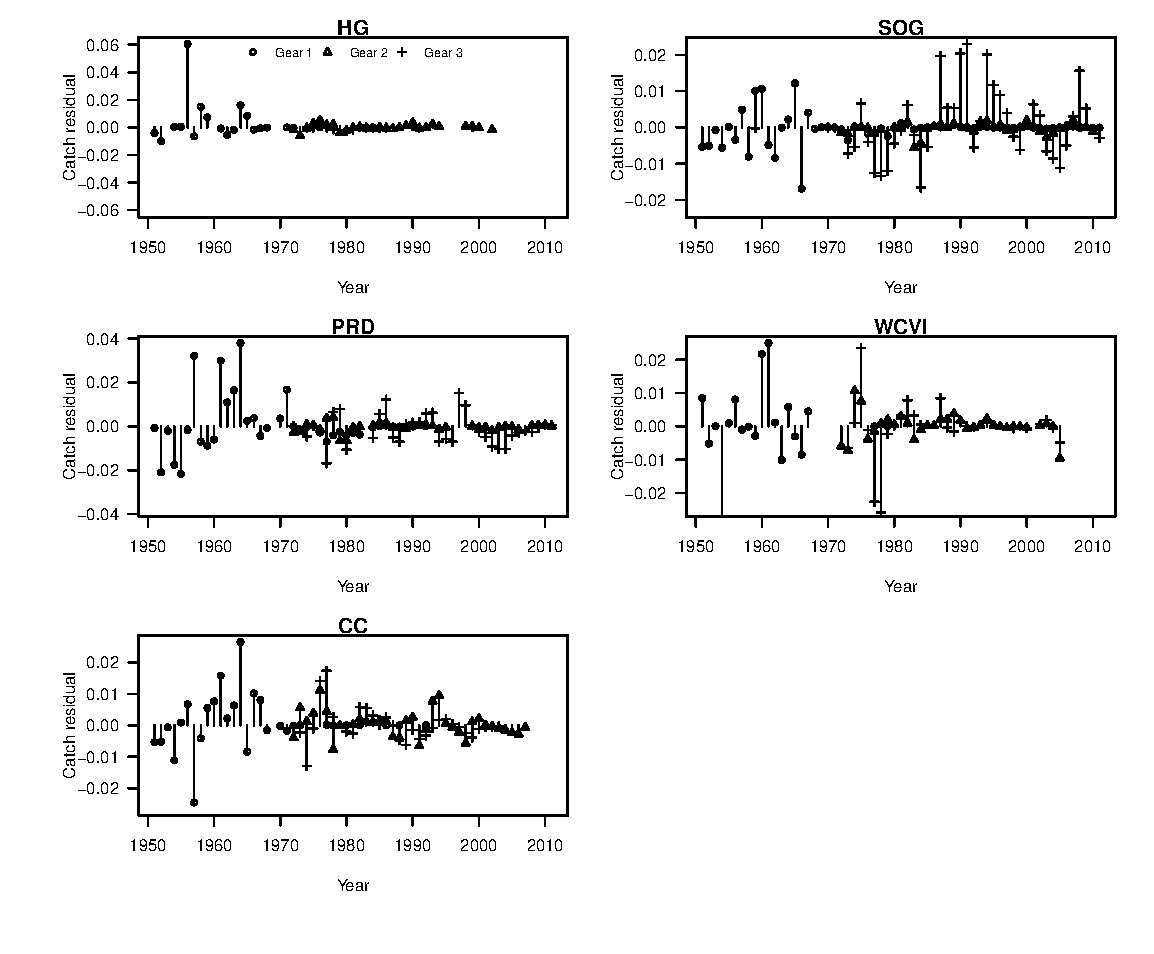
\includegraphics[width=\textwidth]{../FIGS/qPriorFigs/iscam_fig_catchresid.pdf}\\
	\caption{Residual for the log difference between observed and predicted catch for the five major SARs for each gear type (Gear 1 = winter seine fishery, Gear 2 = seine-roe fishery, Gear 3 = gillnet fishery).}\label{PartII:Results:fig1}
\end{figure}


\subsubsection{Fits to the spawn survey data}
The residuals between the observed and predicted spawn survey index (on a log scale) are shown in Figure \ref{PartII:Results:fig2}.  Recall that the spawn survey data are treated as two independent time series where data between 1951--1987 were based on surface estimates of spawn deposition and data post 1988 are based on diver surveys of spawn deposition.  More weight was assigned to the contemporary data.  Also, you might be tempted to compare the estimated values of $q$ in Figure \ref{PartII:Results:fig2} with those estimated in Part I of this document (e.g., Table \ref{Table:HCAM_stats} on page \pageref{Table:HCAM_stats}).  The results in Table \ref{Table:HCAM_stats} are based on data from 1951 to 2010 (i.e., omit the 2011 data) and use a different parameterization of the selectivity function for the gillnet fishery (type 7 as opposed to type 8, see Appendix \ref{Appendix:SelectivityOptions} on page \pageref{Appendix:SelectivityOptions}).

For most areas, there is little pattern in the residuals between the observed and predicted survey data (Fig \ref{PartII:Results:fig2}).  For the HG, PRD and CC regions, there is very good correspondence between the observed and predicted survey data post 1988.  In the SOG, there is a period of positive residuals between 1999 and 2005 where the predicted spawn biomass fails to increase as much as indicated by the survey.  Similary 3--4 year trends also exist in the WCVI spawn survey data after the year 2000.

\begin{figure}[!tbp]
	% Requires \usepackage{graphicx}
	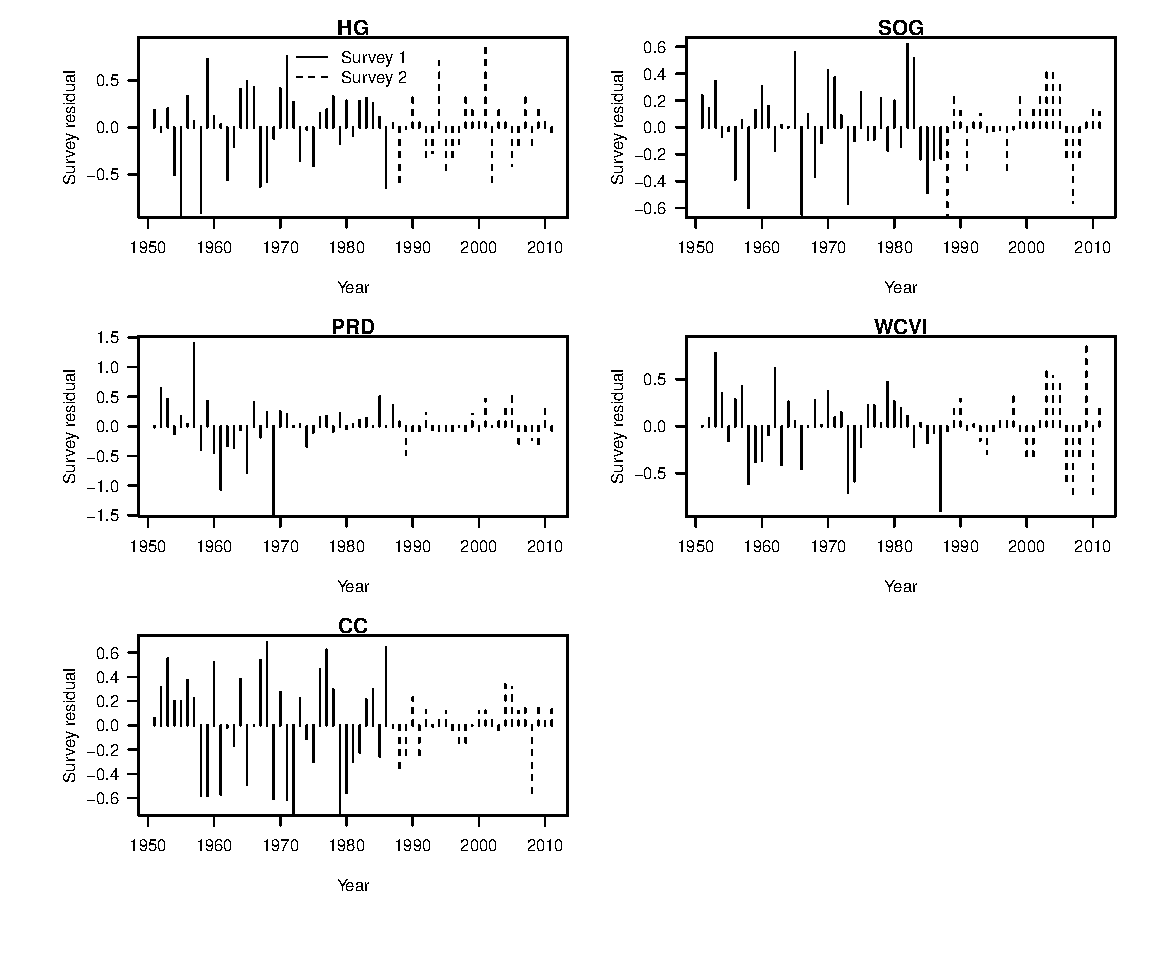
\includegraphics[width=\textwidth]{../FIGS/qPriorFigs/iscam_fig_surveyresid.pdf}\\
	\caption{Residual patterns for the log difference between observed and predicted spawn survey abundance for the five major SARs. Spawn survey data based on surface estimates are show as solid lines and data based on diver surveys is shown as dashed lines.}\label{PartII:Results:fig2}
\end{figure}

In comparison to the previous assessment for Pacific herring using the HCAM model, estimates of the catchability coefficient are very different (HCAM assumed q=1 for post 1988 data).  In each of the five major assessment regions (and the two minor regions) a less informative prior for the catchability coefficient was used (see Appendix \ref{Appendix::q_prior}).  Maximum Likelihood Estimates (MLE) of the catchability coefficients are presented for each region in Fig. \ref{PartII:Results:fig3} along with the observed and predicted trends in the spawn index.  Estimates of $q$ in both time periods are less than 1.0 for all regions.  The interpretation of $q=1$ is that the spawn survey data is an absolute measure of spawn abundance, $q<1$ implies that the survey under-estimates the spawn abundance and $q>1$ implies an over-estimate.  For example, in the HG region the MLE values for $q$ are 0.248 and 0.434 for the pre- and post-1988 data, respectively. This could be interpreted as the spawn survey, on average, sees 24.8\% and 43.4\% of the deposited spawn each year.  This interpretation however is conditional on the specification of mature biomass in the stock assessment model and the methods used to extrapolate egg density to spawning biomass. 

\begin{figure}[!tbp]
	% Requires \usepackage{graphicx}
	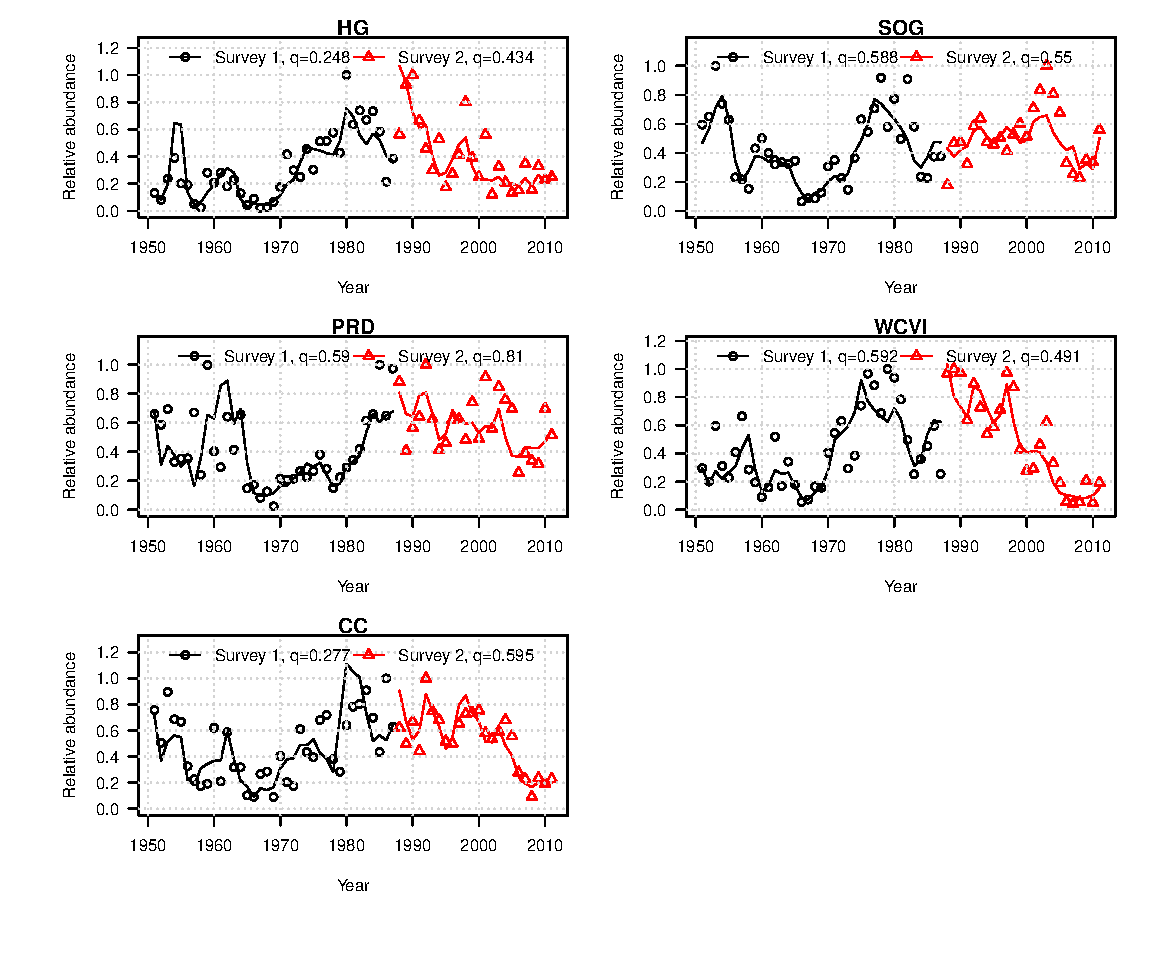
\includegraphics[width=\textwidth]{../FIGS/qPriorFigs/iscam_fig_surveyfit.pdf}\\
	\caption{Observed (points) and predicted (lines) relative abundance data (spawn survey data) for each of the five major SARs.  In each panel, the corresponding scaler ($q$) is presented for each of the surveys.}\label{PartII:Results:fig3}
\end{figure}


\subsubsection{Age composition residuals}

The assumed error distribution for the age-composition data has changed in this assessment from a multinomial distribution implemented in HCAM to a multivariate-logistic distribution. In the former implementation the age-composition data were weighted by the annual samples sizes in each region for each age and year. In the \iscam\ implementation the age-composition data for all years is given the same weight (i.e., we assume the observation errors is homogenous) based on the conditional maximum likelihood estimate of the variance (see Appendix \ref{appiSCAM} for full details).  We further pool age-proportions that are less than 2\% into the adjacent younger year class to reduce the influence of small outliers and weak cohorts.

In HG the MLE estimates of the variance for each gear is 0.102, 0.106 and 0.306, for the winter seine, seine-roe and gillnet fleets, respectively (Fig. \ref{PartII:Results:figAgeCompHG}).  In general there is fairly good agreement between the observed and predicted age-composition data in this region, with poorer fits to the gillnet age-composition data.  There is no persistent pattern in the residuals. 

\begin{sidewaysfigure}[!tbp]
	% Requires \usepackage{graphicx}
	\centering
	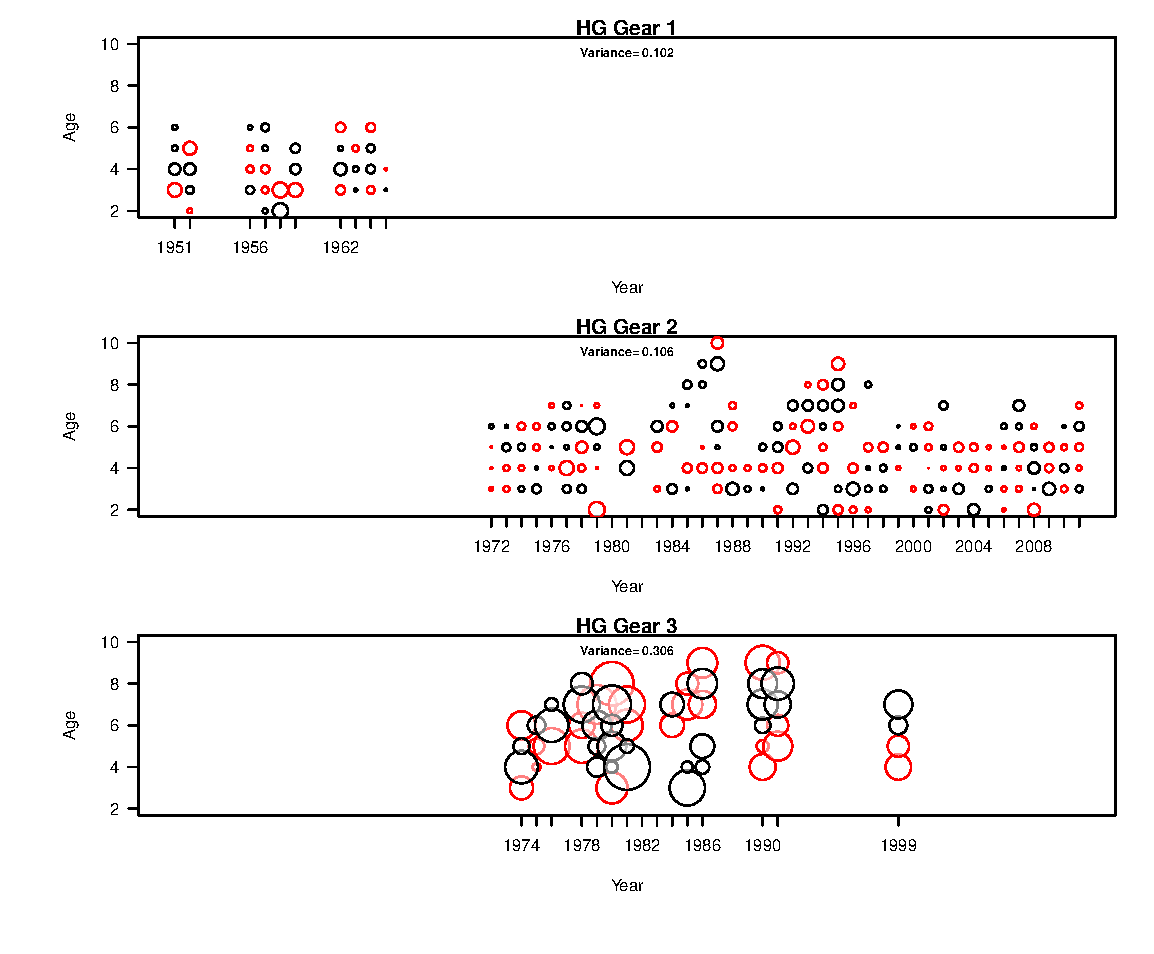
\includegraphics[width=0.9\textwidth]{../FIGS/qPriorFigs/iscam_fig_agecompsresid_HG.pdf}\\
	\caption{Residual difference between the observed and predicted proportions-at-age for HG for each of the three gear types (Gear 1 = winter seine, Gear 2 = seine-roe, Gear 3 = gillnet).  The area of each circle is proportional to the residua, black is positive, and red is negative.  The corresponding MLE estimates of the residual variance is displayed in each panel.}\label{PartII:Results:figAgeCompHG}
\end{sidewaysfigure}

For the PRD region, the fits to the age-composition data are slightly poorer, with MLE estimates of the variance ranging from 0.164 to 0.269 for the gillnet and winter seine fleets (Fig. \ref{PartII:Results:figAgeCompPRD}). There is no remarkable pattern in the winter seine fishery, the seine-roe fishery tends to have positive residuals for age-3 and age 7+ fish, and negative residuals for ages 5-6 fish. Residuals in the gillnet fishery are mostly negative for age-4 fish post 1988. The gillnet gear tends to catch older fish than both seine gears.

\begin{sidewaysfigure}[!tbp]
	% Requires \usepackage{graphicx}
	\centering
	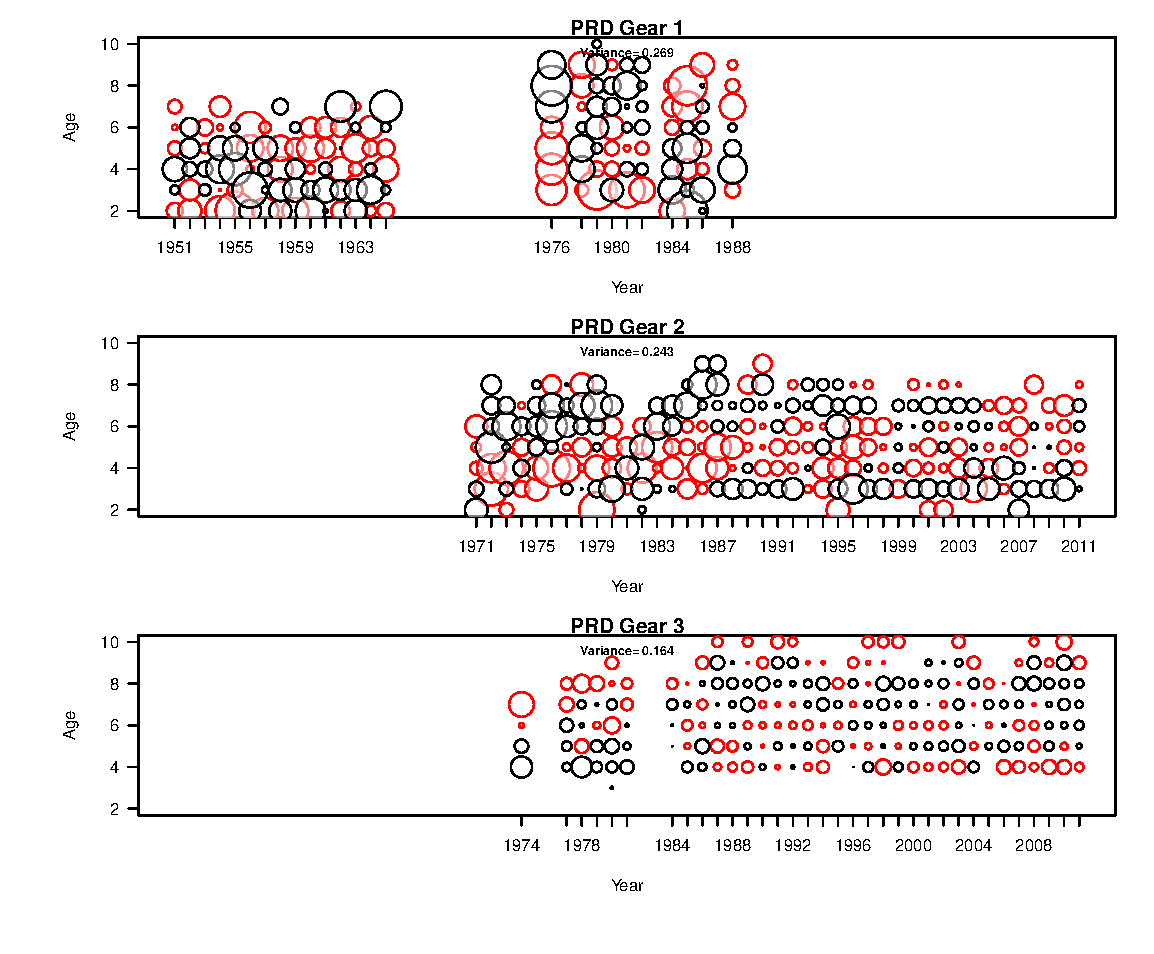
\includegraphics[width=0.9\textwidth]{../FIGS/qPriorFigs/iscam_fig_agecompsresid_PRD.pdf}\\
	\caption{Residual difference between the observed and predicted proportions-at-age for PRD for each of the three gear types (Gear 1 = winter seine, Gear 2 = seine-roe, Gear 3 = gillnet).  The area of each circle is proportional to the residua, black is positive, and red is negative.  The corresponding MLE estimates of the residual variance is displayed in each panel.}\label{PartII:Results:figAgeCompPRD}
\end{sidewaysfigure}


For the Central Coast (CC) region, there is also good correspondence between the observed and predicted age-composition data, with MLE estimates of the variance ranging from 0.135 to 0.201 (Fig. \ref{PartII:Results:figAgeCompCC}).  There is no striking temporal pattern in the residuals for any of the fishing fleets.  There is a tendency to overestimate the proportion-at-age 4 in the seine-roe fishery.


\begin{sidewaysfigure}[!tbp]
	% Requires \usepackage{graphicx}
	\centering
	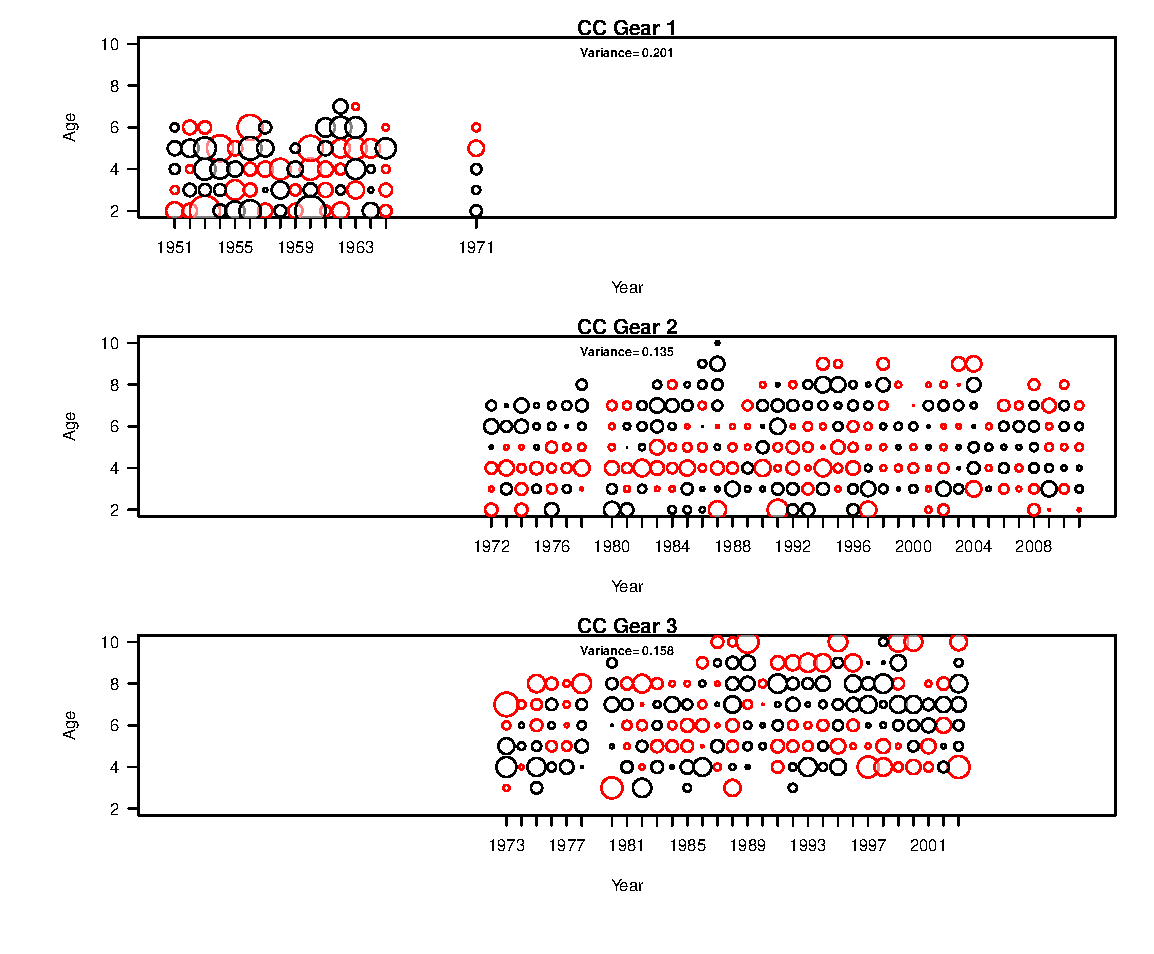
\includegraphics[width=0.9\textwidth]{../FIGS/qPriorFigs/iscam_fig_agecompsresid_CC.pdf}\\
	\caption{Residual difference between the observed and predicted proportions-at-age for CC for each of the three gear types (Gear 1 = winter seine, Gear 2 = seine-roe, Gear 3 = gillnet).  The area of each circle is proportional to the residua, black is positive, and red is negative.  The corresponding MLE estimates of the residual variance is displayed in each panel.}\label{PartII:Results:figAgeCompCC}
\end{sidewaysfigure}

For the Strait of Georgia, there is also very good correspondence between the observed and predicated age-composition data for all three gears (Fig \ref{PartII:Results:figAgeCompSOG}).  The MLE estimates of the variance range from 0.089 to 0.263 for the seine-roe and winter seine fleets, respectively.  In the gillnet fleet  there has been a tendency to under-estimate the proportions-at-age 6-7 between the 1996 to 2011. Recall that selectivity for the gillnet fishery can be influenced by the empirical weight-at-age data, which has been trending to small fish in recent years.  In this case, the age-composition data do not suggest that changes in mean weight-at-age has influenced the selectivity patterns (see results for selectivities).


\begin{sidewaysfigure}[!tbp]
	% Requires \usepackage{graphicx}
	\centering
	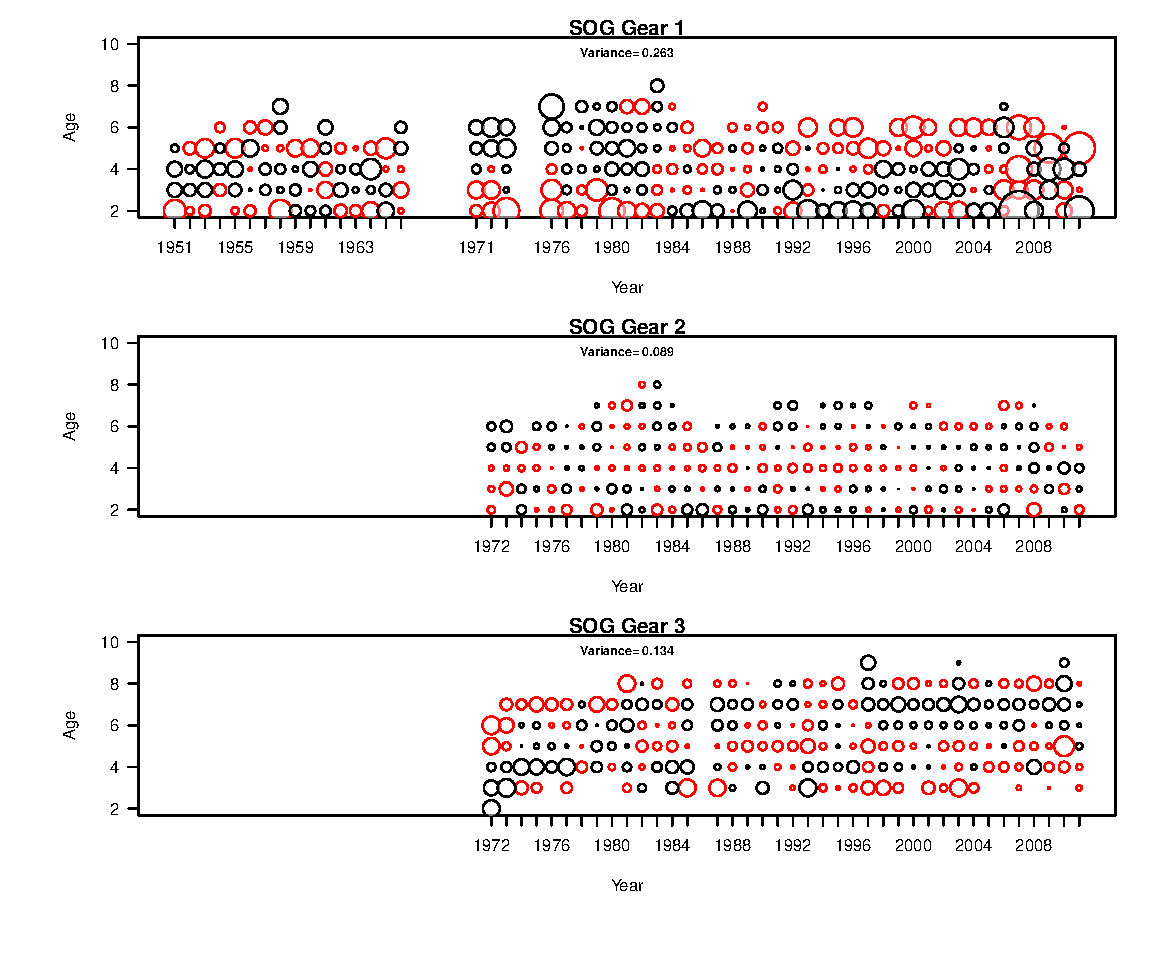
\includegraphics[width=0.9\textwidth]{../FIGS/qPriorFigs/iscam_fig_agecompsresid_SOG.pdf}\\
	\caption{Residual difference between the observed and predicted proportions-at-age for SOG for each of the three gear types (Gear 1 = winter seine, Gear 2 = seine-roe, Gear 3 = gillnet).  The area of each circle is proportional to the residua, black is positive, and red is negative.  The corresponding MLE estimates of the residual variance is displayed in each panel.}\label{PartII:Results:figAgeCompSOG}
\end{sidewaysfigure}

In the case of WCVI, there is good correspondence between the observed and predicted age composition data for the seine fisheries and less so for the gillnet fishery (Fig \ref{PartII:Results:figAgeCompWCVI}).  The MLE estimates of the variance range from 0.092 to 0.237 for the seine-roe and gillnet fisheries, respectively.  Residual patterns in the seine fisheries and gillnet fisheries are unremarkable.   The size of the residuals are fairly homogenous over time for all gears.


\begin{sidewaysfigure}[!tbp]
	% Requires \usepackage{graphicx}
	\centering
	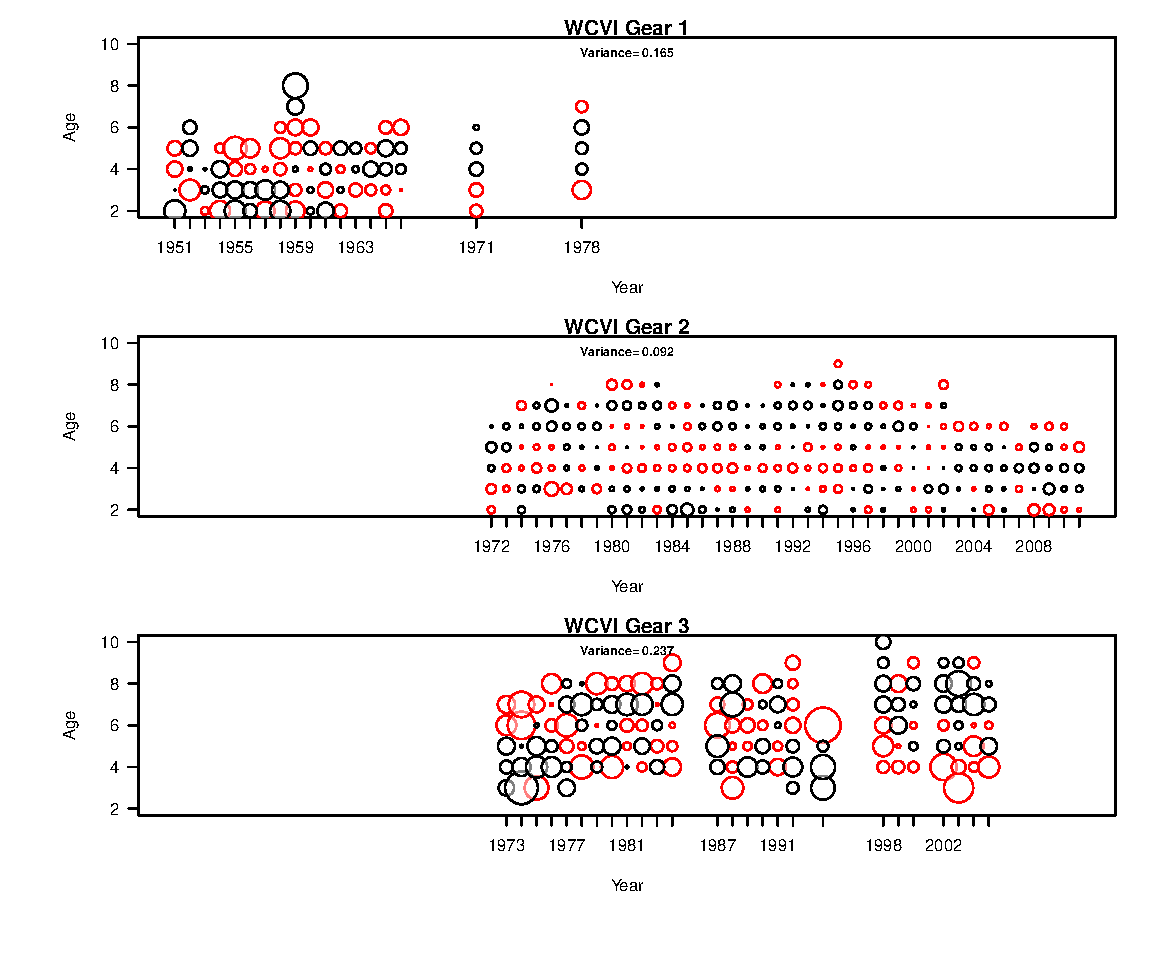
\includegraphics[width=0.9\textwidth]{../FIGS/qPriorFigs/iscam_fig_agecompsresid_WCVI.pdf}\\
	\caption{Residual difference between the observed and predicted proportions-at-age for WCVI for each of the three gear types (Gear 1 = winter seine, Gear 2 = seine-roe, Gear 3 = gillnet).  The area of each circle is proportional to the residua, black is positive, and red is negative.  The corresponding MLE estimates of the residual variance is displayed in each panel.}\label{PartII:Results:figAgeCompWCVI}
\end{sidewaysfigure}







\subsection{Biomass estimates \& reference points}

Maximum likelihood estimates of total biomass (age 2+) and the spawning stock biomass for each of the five major assessment regions in summarized in Figure \ref{PartII:Results:figBiomass}.  Estimates of spawning stock depletion ($B_t/B_0$) for the five major regions is summarized in Figure \ref{PartII:Results:figDepletion} along with estimates of the sustainable fisheries framework reference points.  With the exceptions of CC and WCVI, estimates of spawning stock depletion in 2011 are all currently at or above 40\% of their estimated unfished state. In the  CC and WCVI, spawning stock depletion is estimated to be  25\% and 25\% of their unfished state, respectively (Fig \ref{PartII:Results:figDepletion}).

Maximum likelihood estimates of spawning stock biomass in 2011 were as follows: HG -- 16,723 tonnes, PRD -- 27,288 tonnes, CC -- 14,624 tonnes, SOG -- 129,070 tonnes, and WCVI -- 14,909 tonnes (Table \ref{PartII:Table1:referencePoints}).  These estimates are considerably higher in comparison to last years HCAM estimates; the difference largely owes to the substantial change in spawn survey scaling coefficient ($q$).

In addition to the current estimates of spawning biomass, Table \ref{PartII:Table1:referencePoints} also summarizes estimates of reference points and the total number of estimated parameters for each of the five major stock assessment regions.  Each region contained data from 1951 to 2011, and the number of estimated parameters ranges from 159 in HG to 235 in SOG.  The difference in the number of estimated parameters owes to the difference in the number of years of catch data for each region.

Estimates of unfished spawning biomass for each region is as follows: HG -- 40,684 tonnes, PRD -- 68,761 tonnes, CC -- 59,365 tonnes, SOG -- 135,523 tonnes, and WCVI -- 57,462 tonnes.  Applying the same cuttoff rule used in previous assessments (25\% of $B_0$), results in a substantial change in the cuttoff levels for PRD, CC, SOG, and WCVI.  The previous cuttoff level for HG was estimated at 10,700 tonnes, and in this assessment there is a minor downward revision to 10,171 tonnes.  In the case of PRD, the previous cuttoff was 12,100 tonnes and in this assessment is now 17,190 tonnes.  For the CC, the previous cuttoff was 17,600 tonnes and now 14,841 tonnes.  For the SOG, the previous cuttoff was 21,200 tonnes, and in this assessment it has been revised upwards to 33,881 tonnes.  Lastly, for the WCVI the cuttoff has decreased from 18,800 tonnes to 14,366 tonnes. Note however, that these revised \bo's and cuttoffs are Maximum Likelihood Estimates (MLE) and not median values from the joint posterior distribution (see section \ref{Section:Forecast})


% latex.default(rpTable, file = fn, title = "Stock", longtable = FALSE,      landscape = FALSE, cgroup = NULL, n.cgroup = NULL, caption = cap,      label = "TableRefPoints", na.blank = TRUE, vbar = FALSE,      size = "small") 
%
\begin{table}[!tbp]
 \small
 \caption{Summary of maximum likelihood estimates for  the 
	two minor stock areas.  No. is the total number of estimated 
	parameters, \fmsy\ the average instantaneous fishing rate to 
	achieve the maximum sustainable yield (MSY), \bo\ is the unfished 
	spawning biomass, \bmsy\ is the spawning biomass that achieves 
	maximum sustainable yield,$B_t$ is the spawning biomass at the end 
	of the 2011 fishing season, and $B_t/B_0$ is the spawning depletion 
	level at the end of the 2011 fishing season.\label{TableRefPoints}} 
 \begin{center}
 \begin{tabular}{lll}\hline\hline
\multicolumn{1}{l}{Stock}&\multicolumn{1}{c}{A2W}&\multicolumn{1}{c}{A27}\tabularnewline
\hline
No.&74&79\tabularnewline
\fmsy& 0.34&  1.9\tabularnewline
MSY&  265&  304\tabularnewline
$B_0$&2,915&2,084\tabularnewline
0.25$B_0$&  729&  521\tabularnewline
\bmsy&  705&  447\tabularnewline
0.8\bmsy&  564&  358\tabularnewline
0.4\bmsy&  282&  179\tabularnewline
$B_t$&4,671&  924\tabularnewline
$B_t/B_0$&  1.6& 0.44\tabularnewline
\hline
\end{tabular}

\end{center}

\end{table}




\begin{figure}[!tbp]
	% Requires \usepackage{graphicx}
	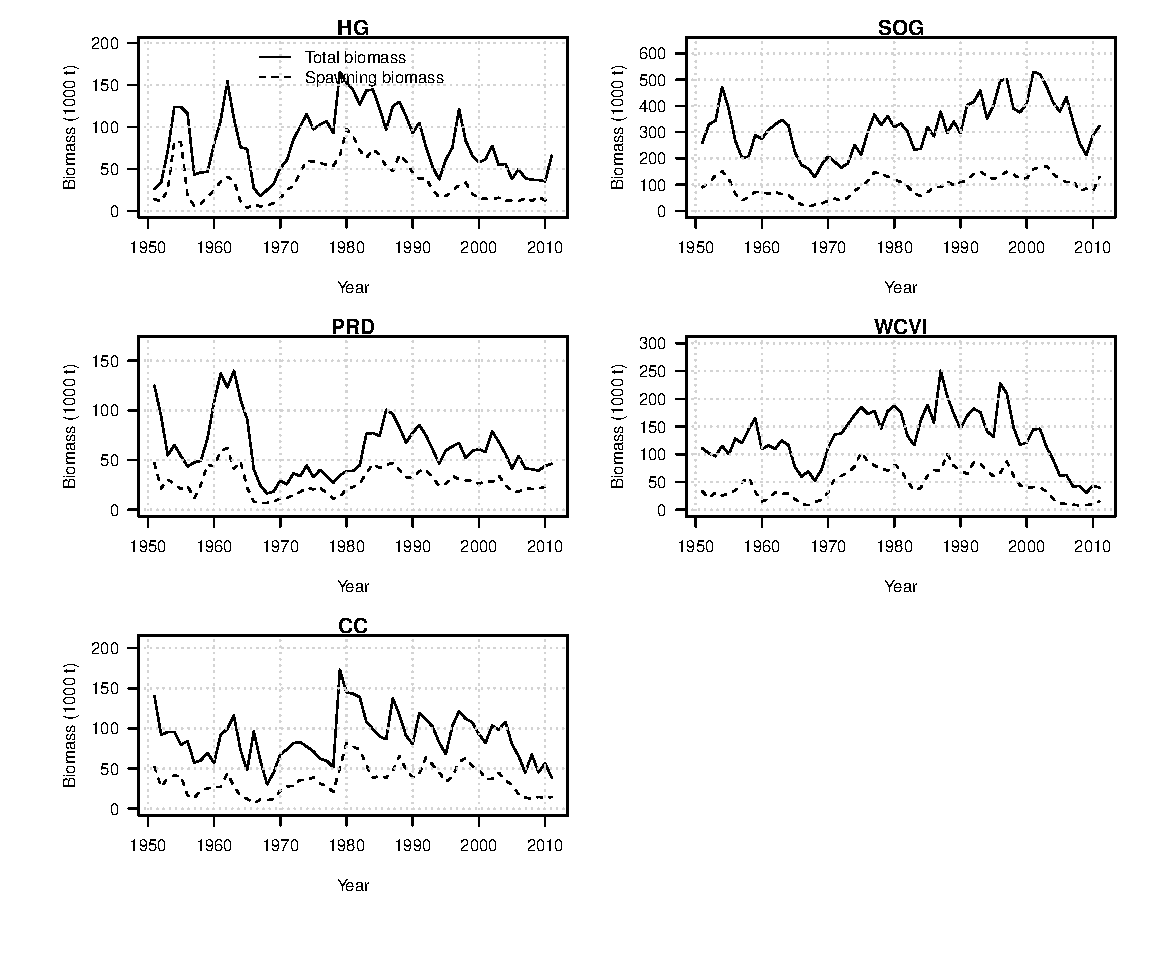
\includegraphics[width=\textwidth]{../FIGS/qPriorFigs/iscam_fig_biomass.pdf}\\
	\caption{Estimates of total biomass at the start of the year (numbers times empirical weight-at-age) and spawning stock biomass (post fishery) for the five major SARs.}\label{PartII:Results:figBiomass}
\end{figure}


\begin{figure}[!tbp]
	% Requires \usepackage{graphicx}
	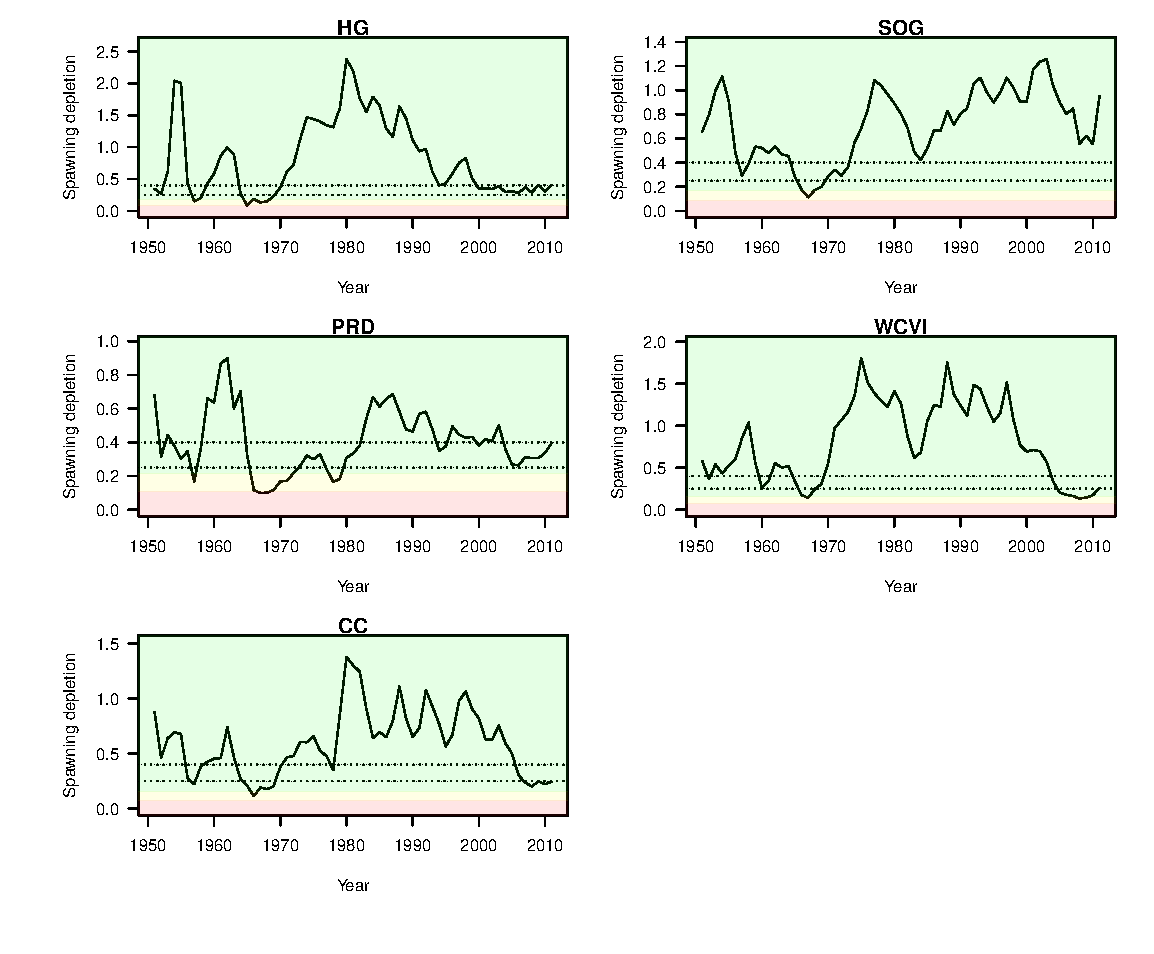
\includegraphics[width=\textwidth]{../FIGS/qPriorFigs/iscam_fig_depletion.pdf}\\
	\caption{Estimates of spawning biomass depletion ($B_t/B_0$) for each of the five major stock areas.  Horizontal dotted lines represent 25\% and 40\% depletion levels, and the shaded regions demarcate reference points based on $<$40\% \bmsy/\bo (critical zone) and 40--80\% \bmsy/\bo(cautious zone) and $>$80\% \bmsy/\bo (healthy zone). Note that \bmsy\ reference points are based on an arbitrary allocation of catch to each of the three gears; changes in allocation would affect estimates of \bmsy.}\label{PartII:Results:figDepletion}
\end{figure}




\subsection{Estimates of mortality}

The most recent HCAM assessment model allowed for annual estimates of $M_t$ where natural mortality was modelled as a random walk process.  The same random walk model has been adopted in this \iscam\ implementation; however, a reduced number of parameters (12 nodes instead of 60 annual deviations) was estimated and interpolated using a bicubic spline.  The number of estimated nodes does have minor influences on the various trends in natural mortality; we came to arrive at estimating 12 nodes by ensuring the estimated trends were very similar to trends in $M$ when estimating 60 annual natural mortality rate deviations (NB. the use of formal model selection criterion should be used to determine the optimal number of nodes).

For all of the five major stock assessment regions, estimates of natural mortality rates have trended upwards since the 1950s (Figure \ref{PartII:Results:figMortality}).  Trends in estimates of natural mortality are also consistent with the trends in natural mortality from last years HCAM model  \citep[see Figure 18 in][]{Clear2010}.  In the mid to late 1970s, estimates of natural mortality rates were very low during a time when most of the stocks were recovering from the earlier reduction fishery.  In the last decade, estimates of natural mortality rates for herring have been at an all time high, and in all locations there is indication that natural mortality rates may be starting to decline. Estimates of $M_t$ in the most recent years, however,  are highly suspect because there are incomplete cohorts to infer estimates of total mortality rates and $M_t$ is also confounded with selectivity.



\begin{figure}[!tbp]
	% Requires \usepackage{graphicx}
	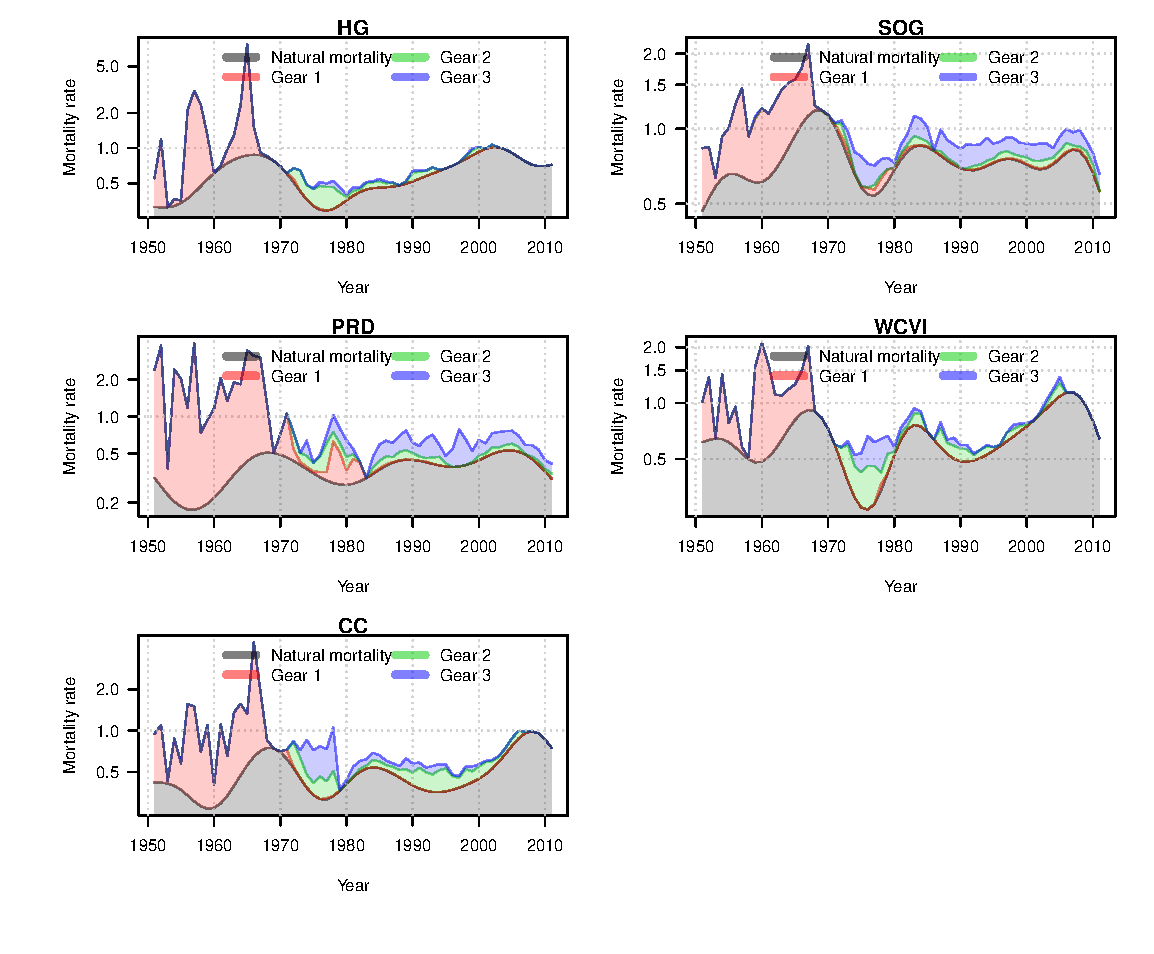
\includegraphics[width=\textwidth]{../FIGS/qPriorFigs/iscam_fig_mortality.pdf}\\
	\caption{Maximum likelihood estimates of the components of average total mortality for each of the five major stock assessment regions. Note that the y-axis is plotted on a log scale, natural mortality (grey) is age-independent, fishing mortality is age-specific and the average fishing mortality rate over all age-classes is plotted here.}\label{PartII:Results:figMortality}
\end{figure}

Estimates of fishing mortality rates in each of the regions, between 1951 and 1970 were very high due to the reduction fishery by the winter purse seine (Gear 1).  After the fishery re-opened in the early 1970s fishing mortality rates have been greatly reduced and periodic since the early 1990s due to the implementation of a harvest control rule with target escapements (cuttoffs).  Of notable exceptions are the fishing mortality rates for the gillnet fishery in PRD  and SOG have been substantially higher than other regions and consistently open each and every year (Fig. \ref{PartII:Results:figMortality}). Note that fishing mortality rates for each gear in Fig. \ref{PartII:Results:figMortality} reflect the average fishing mortality over all age-classes and are not comparable among gears due to differences in gear selectivity. Fishing mortality rates for the gillnet fishery tend to be higher than the seine-roe fishery because recruitment to the gillnet gear is much older in comparison to the seine-roe gear.





\subsection{Selectivity}

Maximum likelihood estimates of selectivity for the winter seine fishery, seine-roe fishery and the gillnet fishery for each of the five major SARs are shown in Figures \ref{PartII:Results:figWinterSeineSel}, \ref{PartII:Results:figSeineRoeSel}, and \ref{PartII:Results:figGillNetSel}, respectively.  Selectivities for the seine fisheries were assumed time-invariant, and selectivity for the gillnet fishery varies over time due to changes in the mean weight-at-age data.

For the winter seine fishery, age-specific selectivity coefficients were somewhat variable among the assessment regions (Fig. \ref{PartII:Results:figWinterSeineSel}).  The age at which herring were fully recruited to the gear was roughly age 5 for CC, SOG, and WCVI.  Age at full recruitment for HG and PRD was much older, 9- and 10-years, respectively.


\begin{figure}[!tbp]
	% Requires \usepackage{graphicx}
	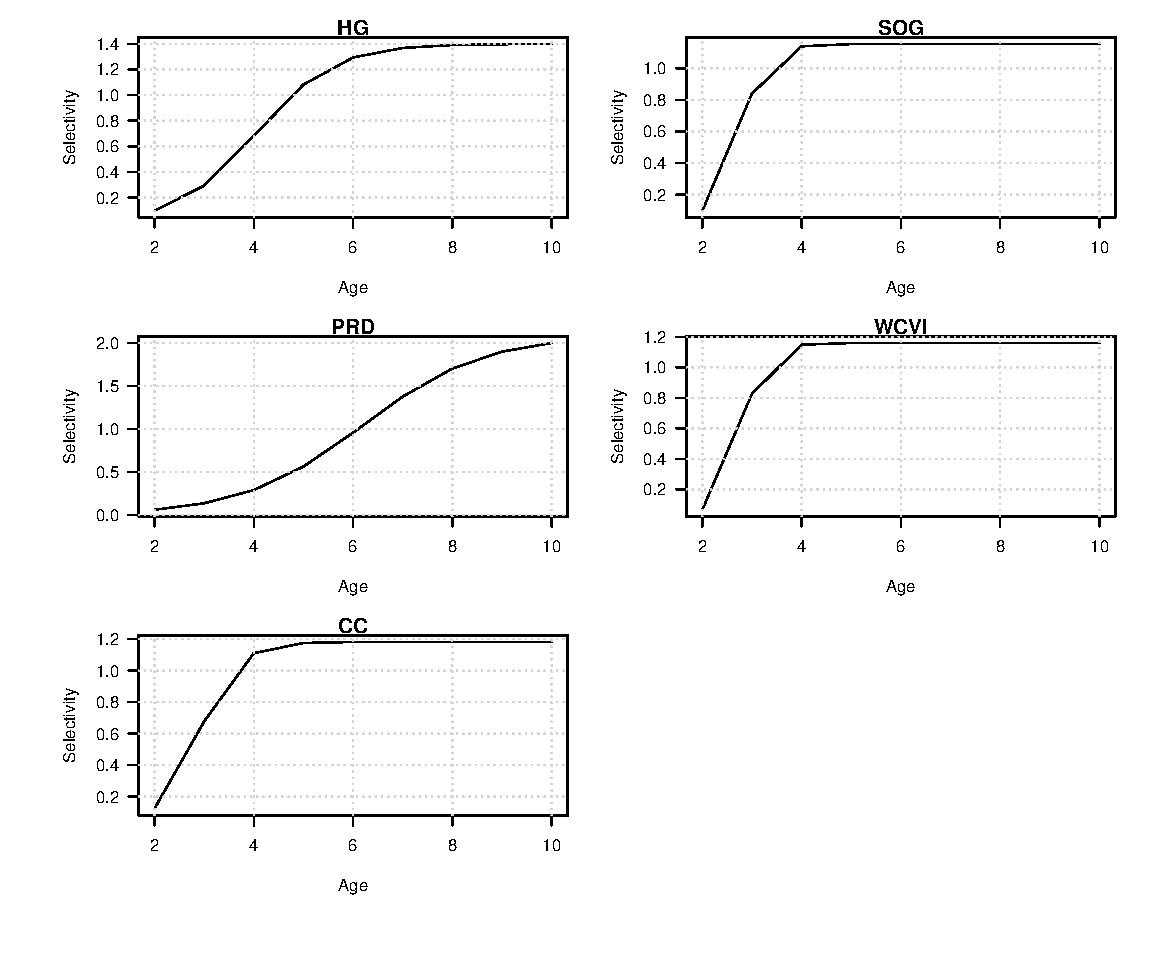
\includegraphics[width=\textwidth]{../FIGS/qPriorFigs/iscam_fig_sel2d_winter_seine_sel.pdf}\\
	\caption{Maximum likelihood estimates of age-specific selectivity coefficients for the winter seine fishery for each of the major stock areas.}\label{PartII:Results:figWinterSeineSel}
\end{figure}

For the seine-roe fishery, maximum likelihood estimates of selectivity were much more consistent among regions than the winter seine fishery (Fig. \ref{PartII:Results:figSeineRoeSel}).  Age at full recruitment to this gear type was roughly 5-6 years, and roughly the age at 50\% vulnerability was roughly 3-4 years, with a tendency to recruit to the fishery at a younger age in the southern regions.

\begin{figure}[!tbp]
	% Requires \usepackage{graphicx}
	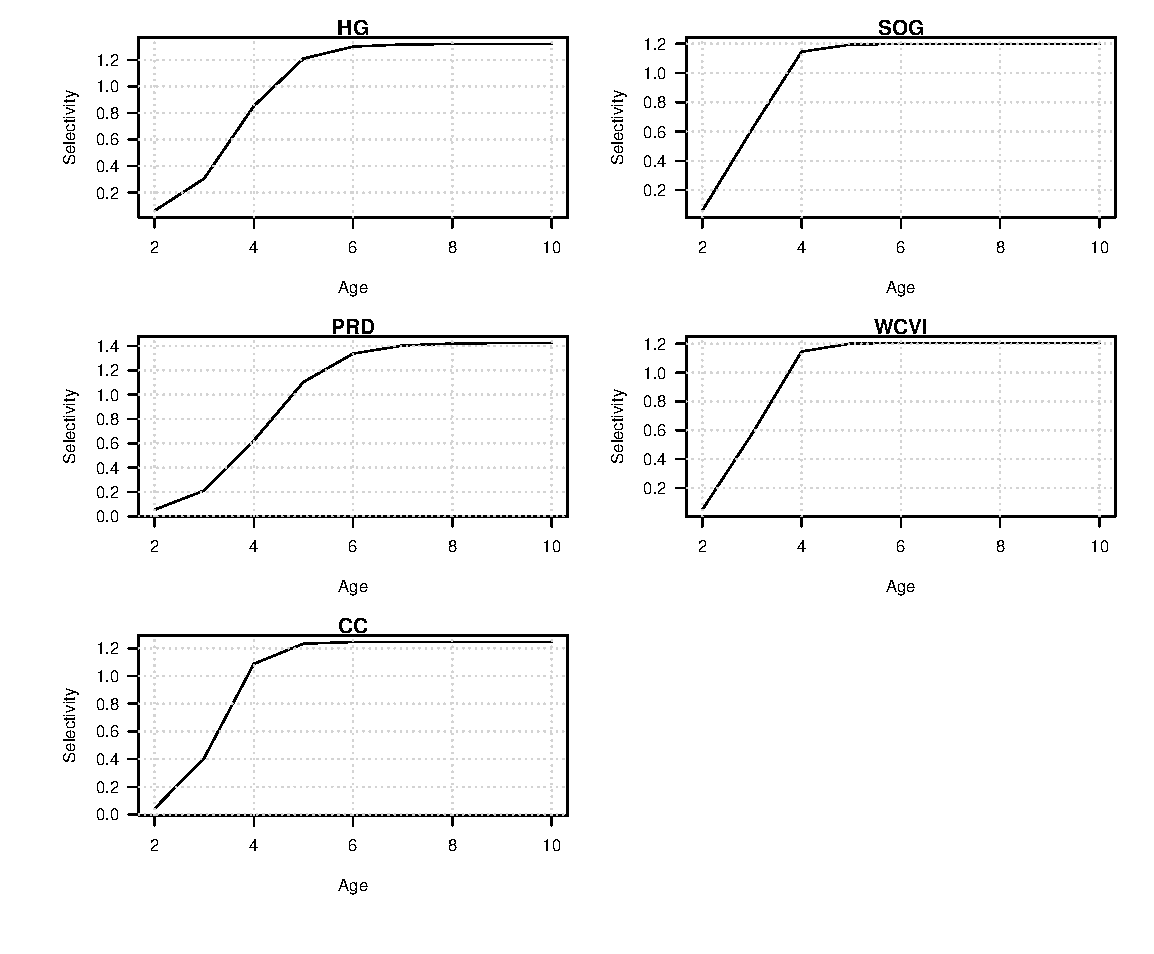
\includegraphics[width=\textwidth]{../FIGS/qPriorFigs/iscam_fig_sel2d_seine_roe_sel.pdf}\\
	\caption{Maximum likelihood estimates of age-specific selectivity coefficients for the seine-roe fishery for each of the major stock areas.}\label{PartII:Results:figSeineRoeSel}
\end{figure}

In the case of the gillnet fishery, selectivity was allowed to vary over time according to variation in the empirical weight-at-age data (Fig. \ref{PartII:Results:figGillNetSel}).  Recall that selectivity for the gillnet fishery was modelled as a logistic function of age with the addition of age-specific deviations where selectivity can increase if the weight-at-age is above average for that year.  This selectivity function consists of three latent variables: two that describe the age-at-50\% vulnerability and standard deviation in vulnerability-at-age, and a third parameter that describes the influence of variation in weight-at-age on departures from the logistic selectivity function ($\lambda^{(a)}$).  Maximum likelihood estimates for these parameters for the gillnet fishery are presented in Table \ref{PartII:Table:GN_Sel_par}.  With the exception of PRD and WCVI, estimates of $\lambda^{(a)}$ are negative and close to 0 implying no affect of variation in weight-at-age on selectivity or a slight negative effect (i.e., vulnerability to the gear declines for fish that are larger than the average weight).  In the case of PRD and WCVI, the variation in weight-at-age explains approximately 4.1\% and 8.7\% of the residual variation in the age-composition data (Table \ref{PartII:Table:GN_Sel_par}).

\begin{figure}[!tbp]
	% Requires \usepackage{graphicx}
	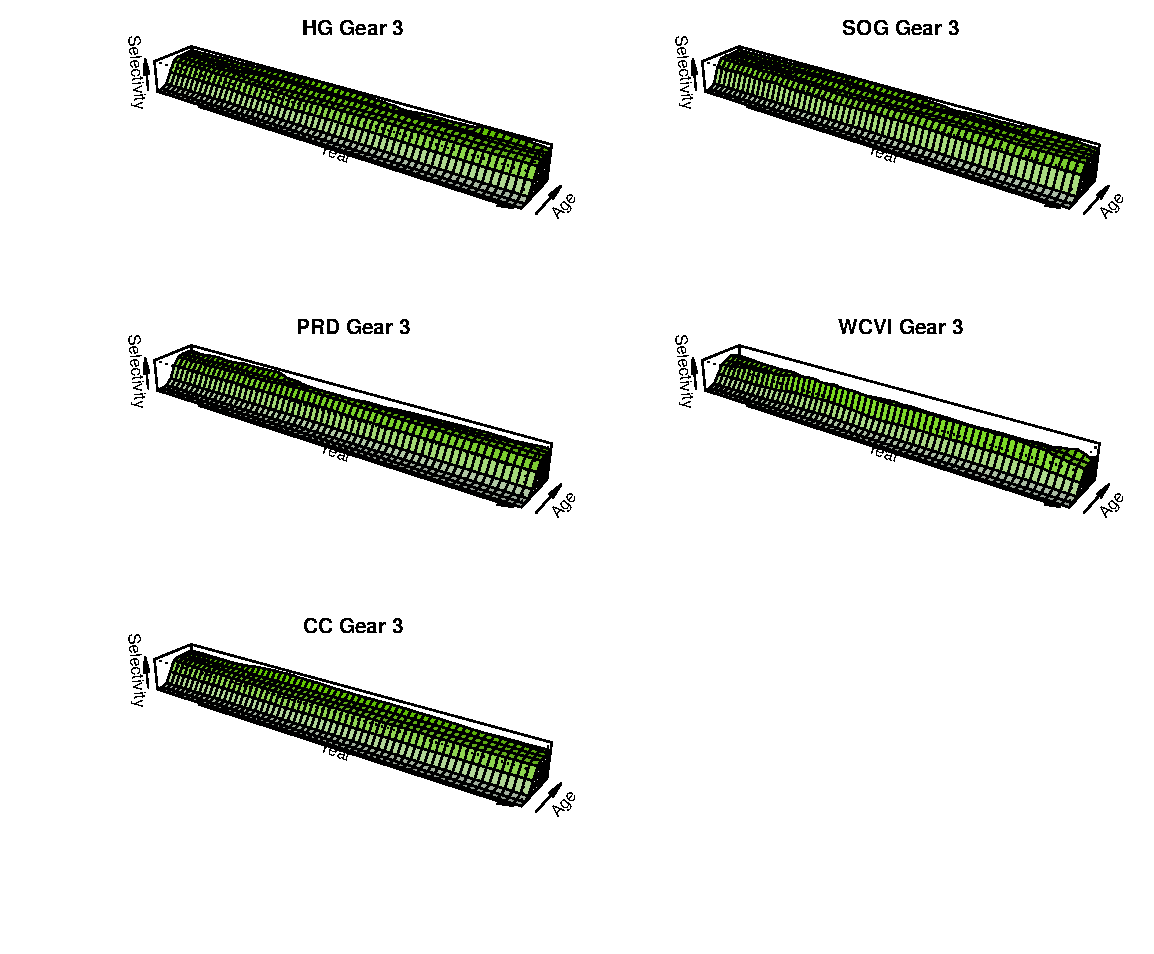
\includegraphics[width=\textwidth]{../FIGS/qPriorFigs/iscam_fig_gill_net_selectivity.pdf}\\
	\caption{Estimates of selectivity for the gillnet fleet for each of the five major stock assessment regions. In this case selectivity is a logistic function of the empirical weight-at-age data; due to declining growth there is a tendency for selectivity to shift to older ages.}\label{PartII:Results:figGillNetSel}
\end{figure}


%% Insert table here with estimates of selectivity parameters.
\begin{table}[htdp]
\caption{Maximum likelihood estimates of gillnet selectivity parameters, where $\mu_a$ is the age-at-50\% vulnerability, $\sigma_a$ is the standard deviation in selectivity, and $\lambda^{(a)}$ is the coefficient that describes the influence of growth on selectivity ($\lambda^{(a)}$=0 implies no effect, $\lambda^{(a)}>0$ implies a positive effect).}
\begin{center}
\begin{tabular}{lccc}
\hline
Stock 	& $\ln(\mu_a)$ 	& $\ln(\sigma_a)$	& $\lambda^{(a)}$ \\
\hline
HG		&	 1.598		&	-0.68125		&	-0.030581	\\
PRD		&    1.727		&   -0.66217		&    0.040988 \\
CC		&    1.604 		&   -0.8050        &   -0.019404\\
SOG		&	 1.540		&   -0.9797			&   -0.02835\\
WCVI	& 	 1.608		&   -0.6647			& 	 0.08677\\
\hline
\end{tabular}
\end{center}
\label{PartII:Table:GN_Sel_par}
\end{table}%


%%%%%%%%%%%%%%%%%%%%%%%%%%%%%%%%%%%%%%%%%%%%%%%%%%%%%%%%%%%%%%%
%%%%%%%%%%%%%%%%%%%%%%%%%%%%%%%%%%%%%%%%%%%%%%%%%%%%%%%%%%%%%%%
\subsection{Recruitment and stock-recruitment relationships}

Recruitment to each stock is defined as the number of age-2 fish entering the population at the beginning of each year. Age-2 recruitment is estimated as a free parameter within \iscam, subject to the constraint that annual estimates vary around a Beverton-Holt stock recruitment relationship with an estimated standard deviation.  Maximum likelihood estimates of age-2 recruits are shown in Figure \ref{PartII:Results:FigAge2Recruits} along with horizontal lines that demarcate the 0.33 and 0.66 quantiles that was traditionally used to categorize recruitment as poor, average, and good in previous assessments.

Estimates of age-2 recruits for 2010 and 2011 were average and good  in HG, average in PRD, good and average in CC, good in SOG, and average and poor in the WCVI region.


\begin{figure}[!tbp]
	% Requires \usepackage{graphicx}
	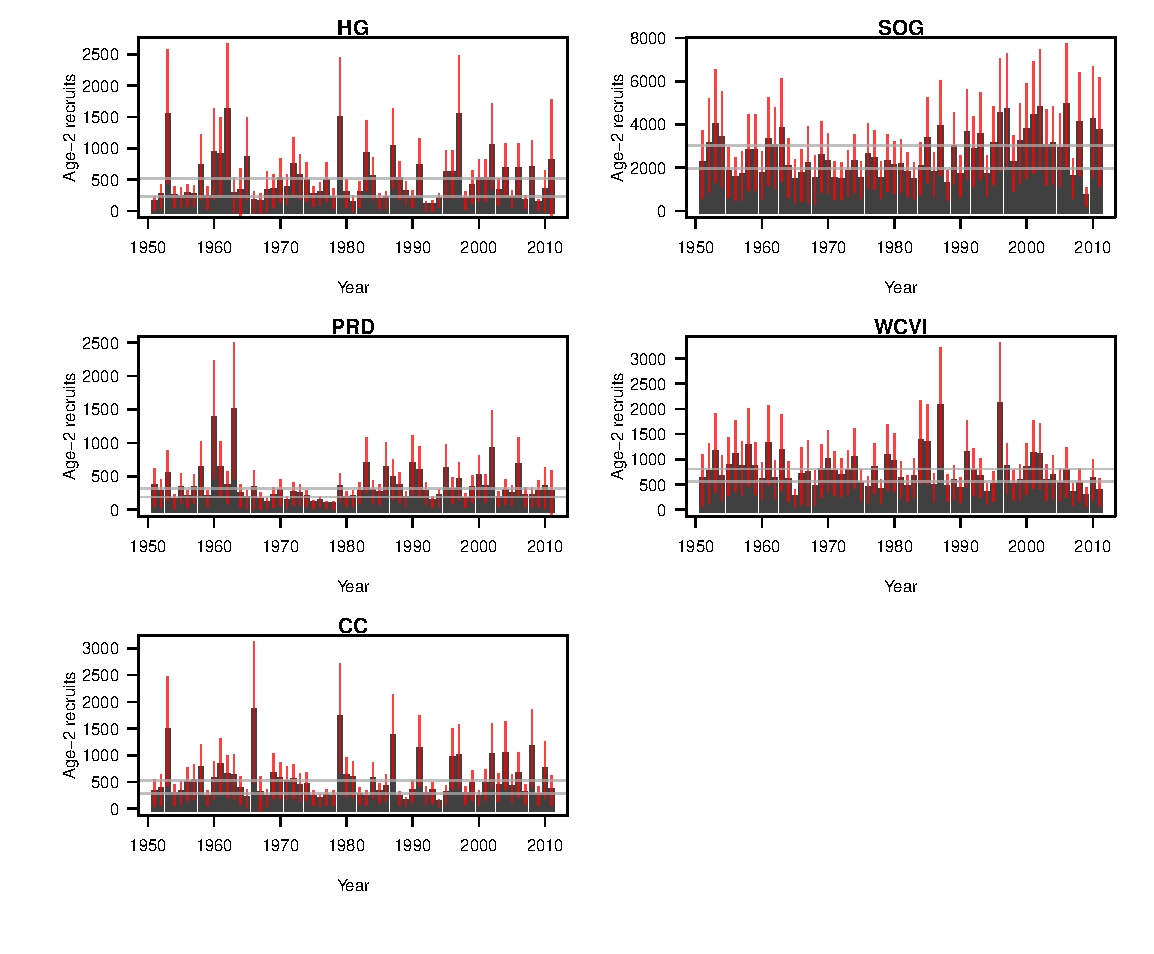
\includegraphics[width=\textwidth]{../FIGS/qPriorFigs/iscam_fig_recruitment.pdf}\\
	\caption{Maximum likelihood estimates of age-2 recruits for each of the five major stock areas.  The horizontal divisions demarcate the 0.33 and 0.66 quantiles that define poor, average, and good recruitment.}\label{PartII:Results:FigAge2Recruits}
\end{figure}

The underlying stock-recruitment relationship is key for determining reference points for this stock.  Maximum likelihood estimates of the age-2 recruits versus spawning biomass, along with the corresponding Beverton-Holt stock recruitment model are shown in Figure \ref{PARTII:Results:FigStockRecruit}.  The Beverton-Holt stock recruitment model was jointly fitted to these data by estimating the steepness of the stock recruitment relationship ($h$) and the unfished age-2 recruits ($R_0$).  The unfished spawning biomass was determined by using the average fecundity and average natural mortality rates (from 1951-2011) to calculate the average spawning biomass per recruit. Alternative stock-recruitment models (e.g., Ricker model) were not explored to determine if they provided a better fit.



\begin{figure}[!tbp]
	% Requires \usepackage{graphicx}
	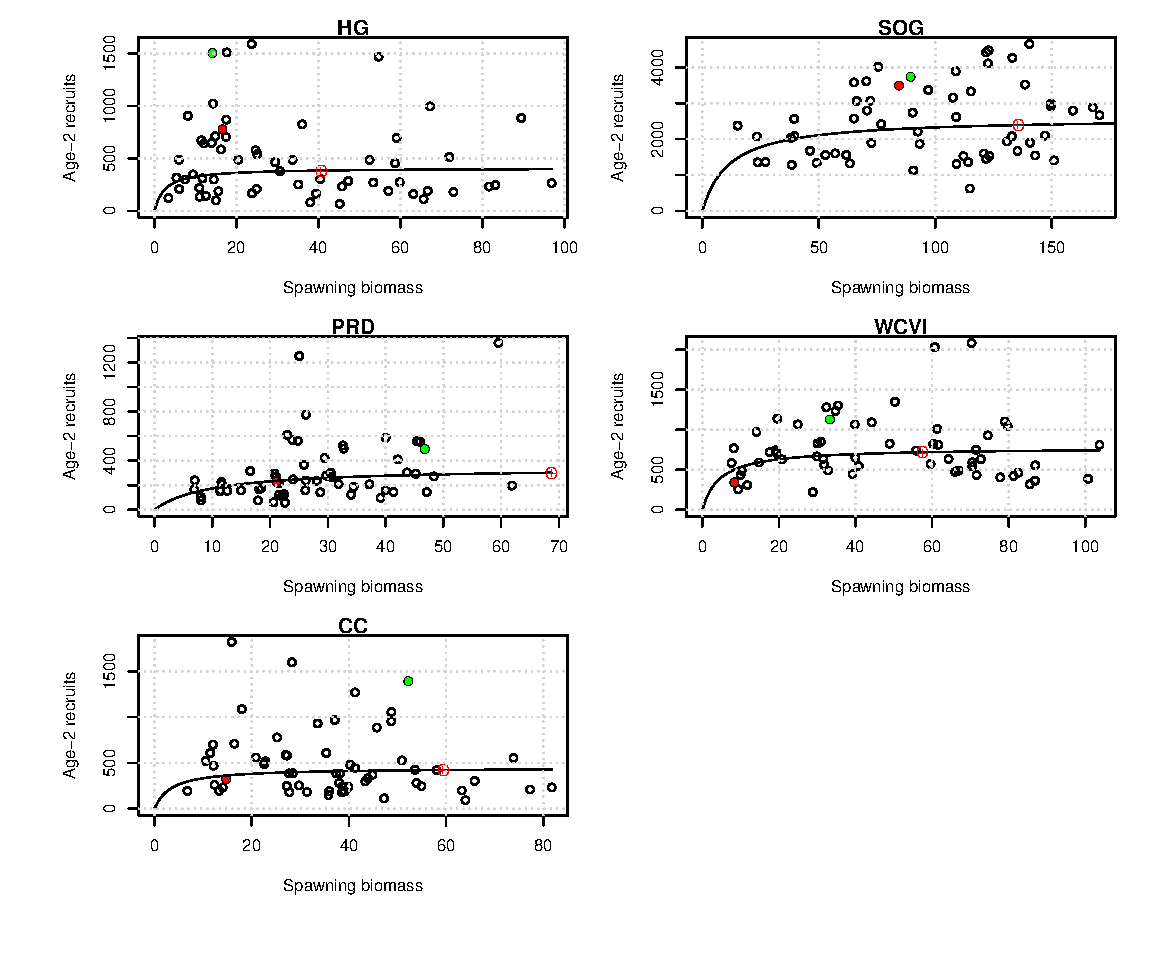
\includegraphics[width=\textwidth]{../FIGS/qPriorFigs/iscam_fig_stockrecruit.pdf}\\
	\caption{Maximum likelihood estimates of age-2 recruits versus estimated spawning stock biomass in each of the five major assessment regions.  The green and red circles indicate the start (recruits in 1952) and end (recruits in 2011) of the series, the circle plus (red) corresponds to the maximum likelihood estimate of unfished spawning biomass (\bo) and unfished age-2 recruitment $R_0$, the line is the Beverton-Holt stock recruitment model fitted to these data. }\label{PARTII:Results:FigStockRecruit}
\end{figure}

Between 1951 and 2011, four of the five major stock areas have fluctuated above the estimate of unfished spawning biomass; the exception is the PRD area.  In HG, age-2 recruitment has been remarkably stable over a very wide range of spawner abundance. This is also the case for CC and WCVI.  In PRD and SOG, variation in recruitment appears to be lower at low spawning abundance and the average recruitment rate tends to drop.  Maximum likelihood estimates for steepness for these five stocks are as follows: HG -- 0.81, PRD -- 0.66, CC -- 0.82, SOG -- 0.76, WCVI -- 0.77.

The log residual differences between the estimated age-2 recruits and that predicted by the estimated spawning-biomass and Beverton-Holt model for each of the major stock areas is shown in Figure \ref{PartII:Results:RecResiduals}.  There is no strong autocorrelation in recruitment, except perhaps 5-8 year periods of poor and good recruitment in SOG.  There is good correspondence between the standard deviations of the residuals and the estimated standard deviation of the process error variance ($\tau$).

\begin{figure}[!tbp]
	% Requires \usepackage{graphicx}
	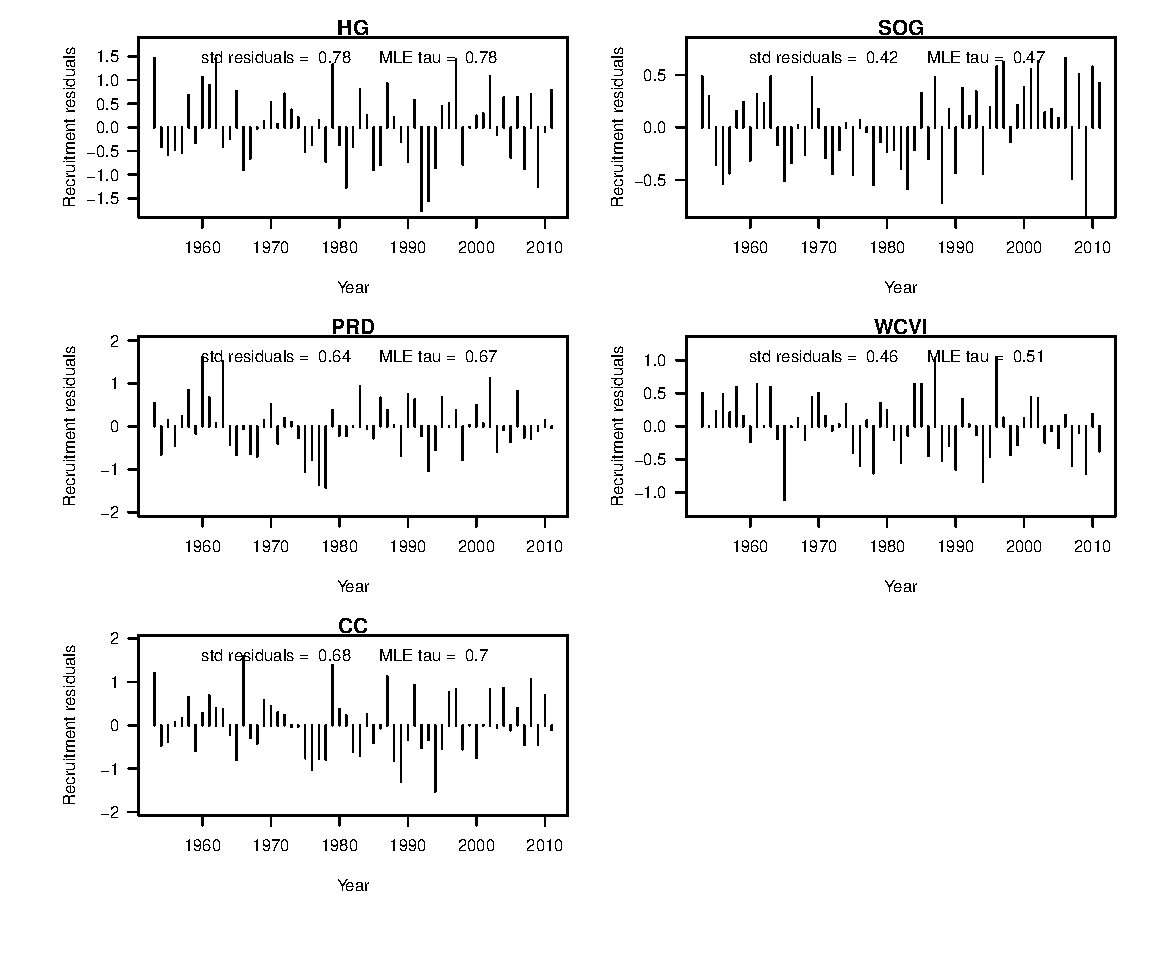
\includegraphics[width=\textwidth]{../FIGS/qPriorFigs/iscam_fig_recresid.pdf}\\
	\caption{Log residual differences between estimated age-2 recruits and the recruitment predicted by the Beverton-Holt model and estimated spawning stock biomass.  The standard deviations of the residuals along with the MLE estimate of the process error standard deviations are displayed at the top of each panel.}\label{PartII:Results:RecResiduals}
\end{figure}
%%%%%%%%%%%%%%%%%%%%%%%%%%%%%%%%%%%%%%%%%%%%%%%%%%%%%%%%%%%%%%%
%%%%%%%%%%%%%%%%%%%%%%%%%%%%%%%%%%%%%%%%%%%%%%%%%%%%%%%%%%%%%%%
\subsection{Retrospective analysis}
Four of the five major regions contained little to no retrospective bias in the estimates of spawning stock biomass when fitting the data back to 2001 (10 years, Figure \ref{fig:PartII:sbRetrospective}).  The PRD region does show a strong retrospective bias; as each year of data is removed estimates of the terminal spawning biomass that year increase.  This pattern of declining estimates of biomass as data are added is persistent for all of the years in which the retrospective estimates were examined.


\begin{figure}[!tbp]
	% Requires \usepackage{graphicx}
	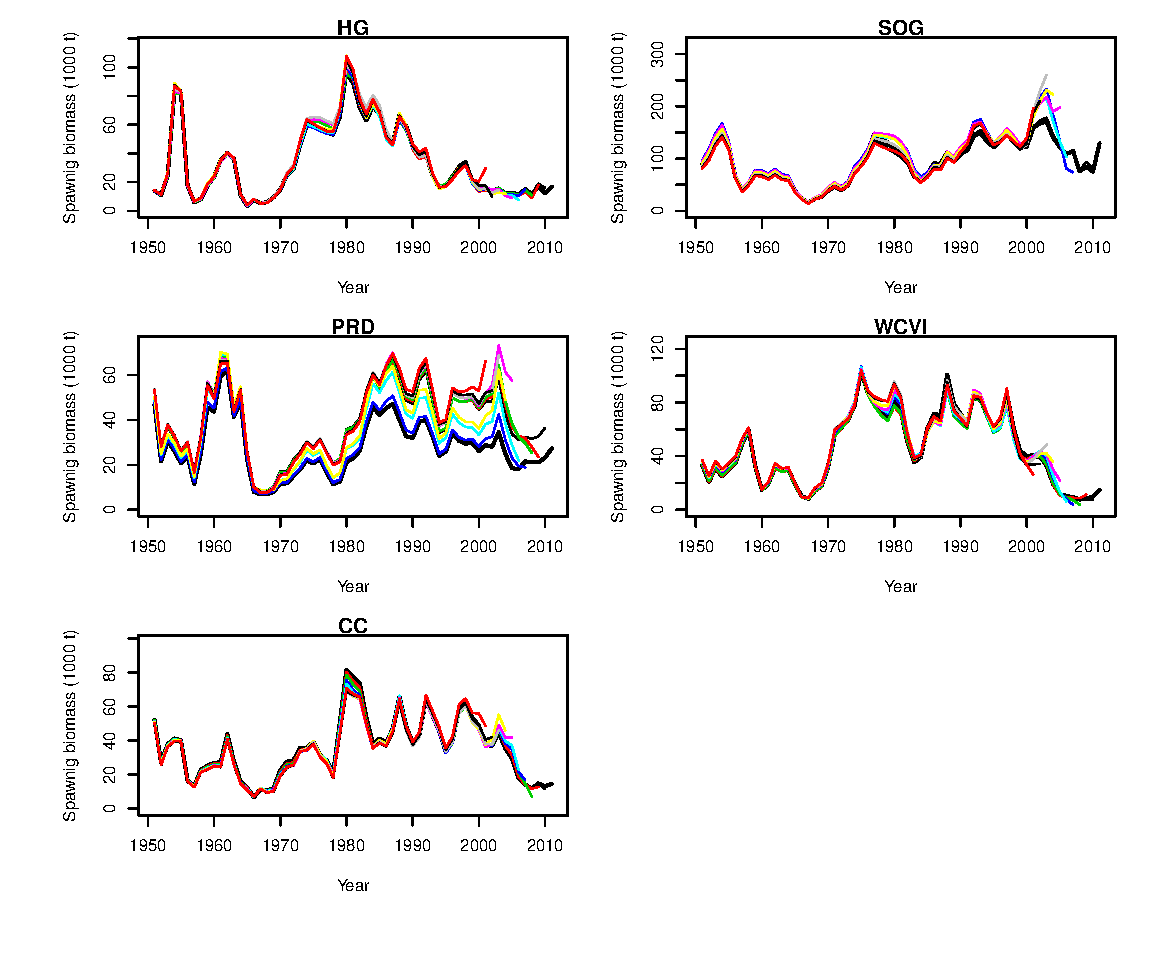
\includegraphics[width=\textwidth]{../FIGS/qPriorFigs/iscam_fig_sbt_retrospective.pdf}\\
	\caption{Retrospective estimates of spawning stock biomass for each of the five major stock assessment areas.  The model was sequentially fitted to the full data set, then from 1951:2010, 1951:2009, ... 1951:2001.}\label{fig:PartII:sbRetrospective}
\end{figure}


%%%%%%%%%%%%%%%%%%%%%%%%%%%%%%%%%%%%%%%%%%%%%%%%%%%%%%%%%%%%%%%
%%%%%%%%%%%%%%%%%%%%%%%%%%%%%%%%%%%%%%%%%%%%%%%%%%%%%%%%%%%%%%%
\subsection{Marginal posterior distributions}
Marginal posterior distributions for estimated model parameters were constructed using AD Model Builders built in Metropolis-Hastings algorithm \citep{gelman2004bayesian}.  For each of the major and minor assessment areas, a systematic sample of 2,000 points from a chain of length 1,000,000 and is intended to represent a random sample from the joint posterior distribution.  These samples were then used to construct marginal distributions for derived quantities (e.g., \bo).  All areas with the exception of the SOG used the inverse Hessian matrix as the jumping distribution.  In the case of SOG, the hessian matrix had to be re-scaled (using the \texttt{-mcmult 2.0} option in ADMB) in order to invert the Hessian matrix.


\subsubsection{Diagnostic trace plots}

No formal  statistical tests were carried out to determine if the samples from the joint posterior distribution were taken from a converged distribution.  Visual inspection was used to determine overall convergence and the trace plots for each of the five major regions are shown in Figures \ref{PartII:MCMC:traceHG}--\ref{PartII:MCMC:traceWCVI}.

\begin{sidewaysfigure}[!tbp]
	% Requires \usepackage{graphicx}
	\centering
	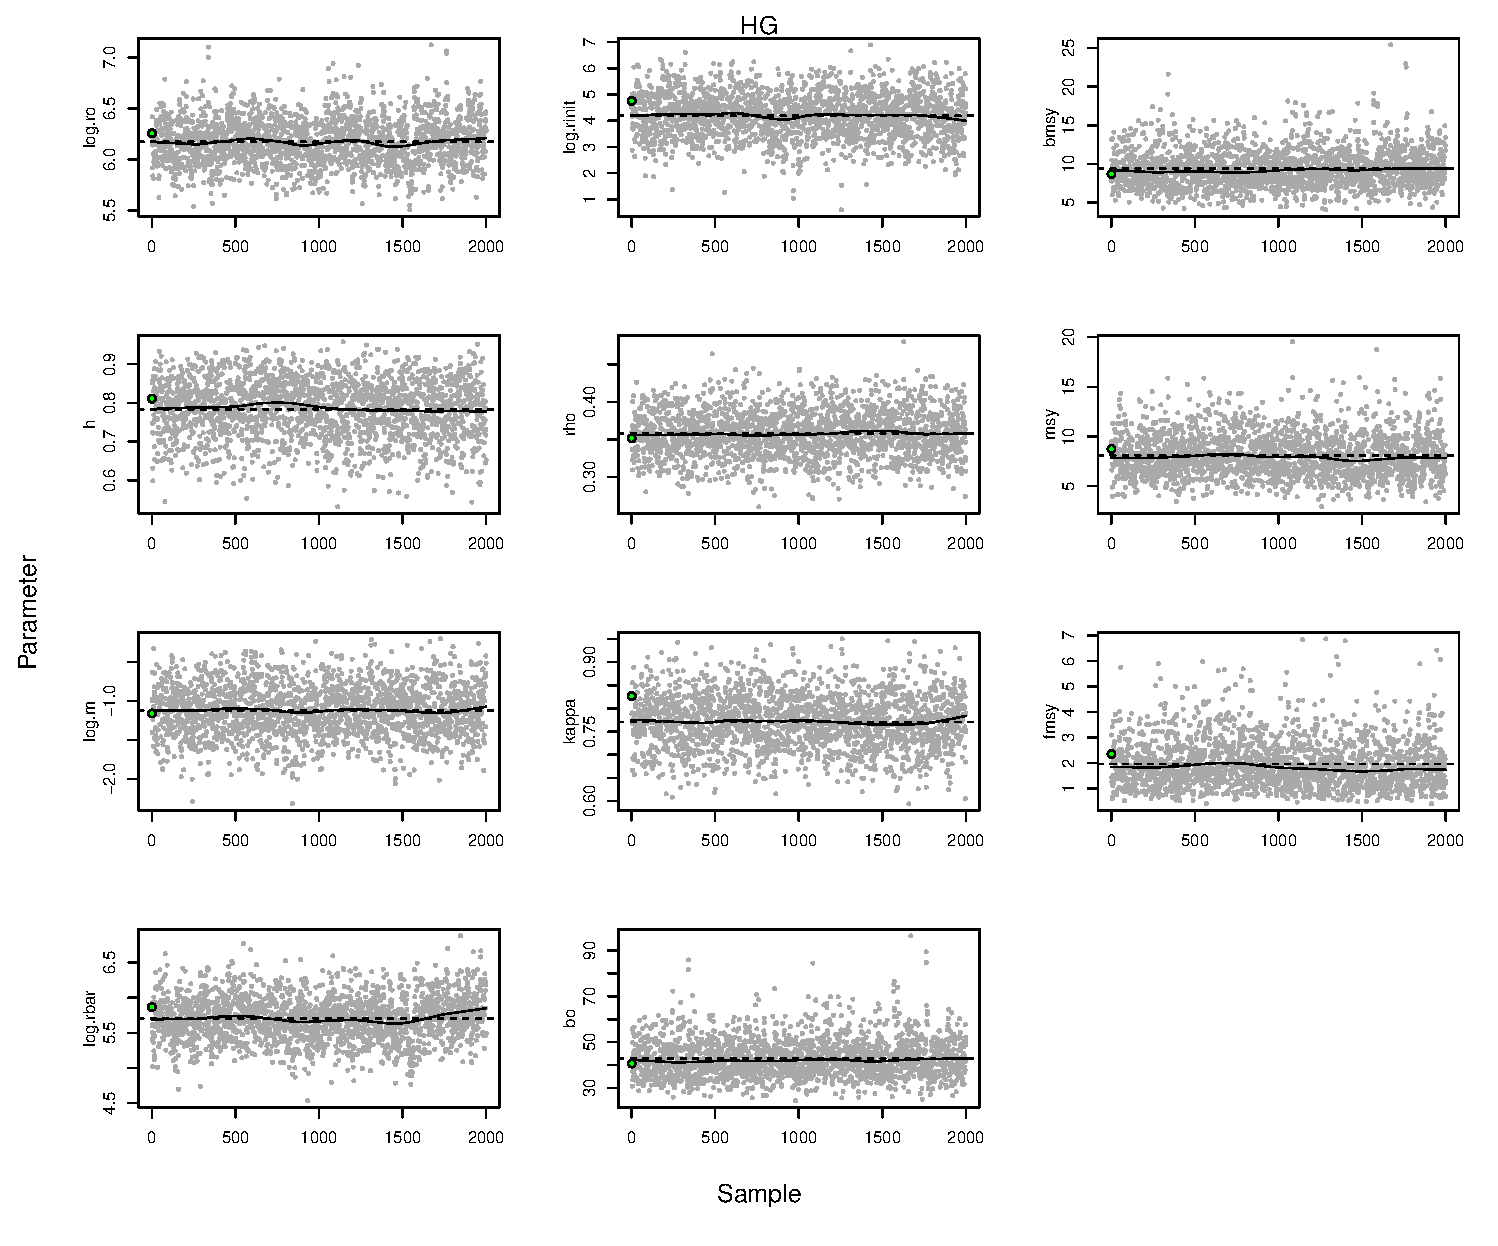
\includegraphics[width=0.9\textwidth]{../FIGS/qPriorFigs/iscam_fig_trace_HG.pdf}\\
	\caption{A systematic sample of 2,000 from an MCMC chain of length 1,000,000 of leading parameters and derived variables used in reference point calculations for HG. Green circle corresponds to the MLE estimates and the solid line is a lowess smooth fit to the data (f=1/4), and the dashed line is the mean of the distribution.}\label{PartII:MCMC:traceHG}
\end{sidewaysfigure}


\begin{sidewaysfigure}[!tbp]
	% Requires \usepackage{graphicx}
	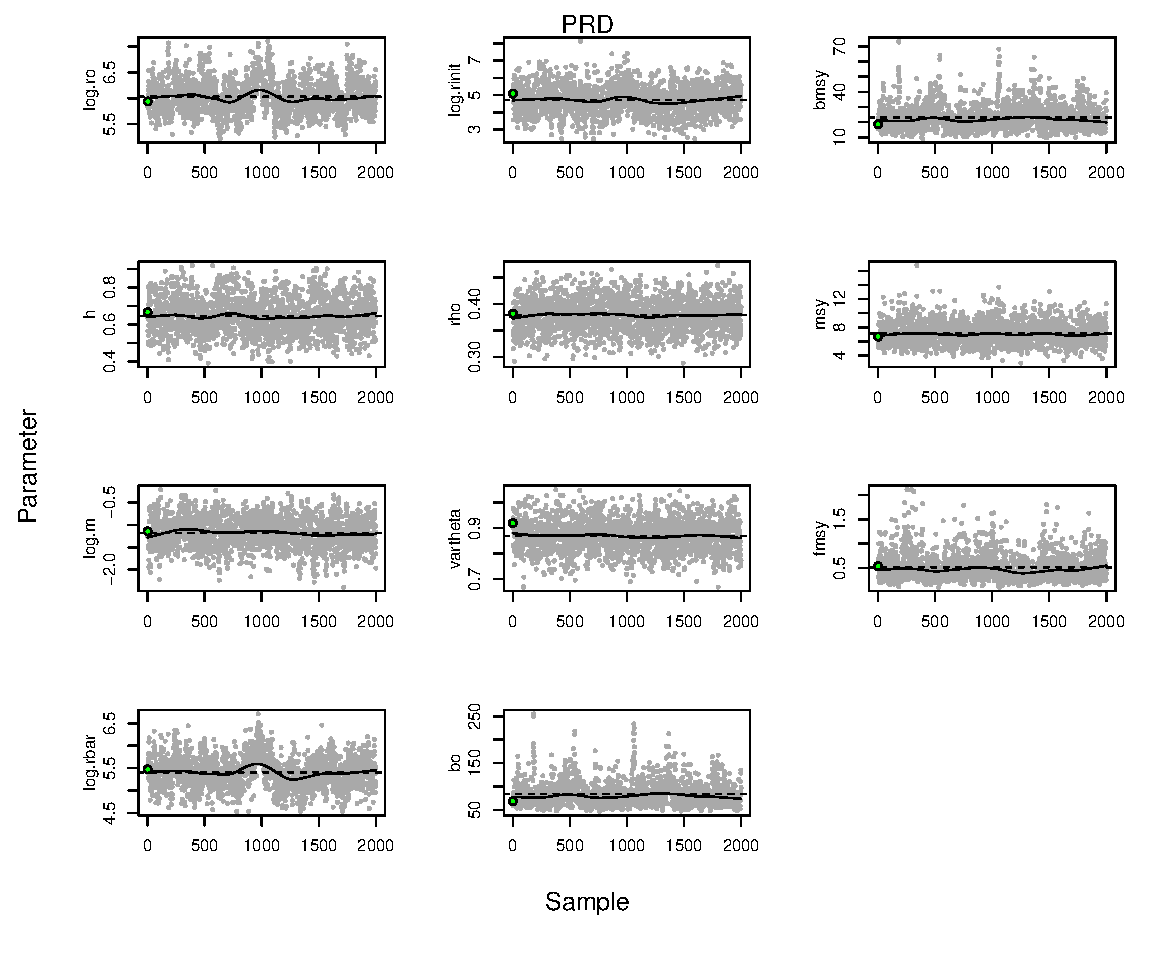
\includegraphics[width=0.9\textwidth]{../FIGS/qPriorFigs/iscam_fig_trace_PRD.pdf}\\
	\caption{A systematic sample of 2,000 from an MCMC chain of length 1,000,000 of leading parameters and derived variables used in reference point calculations for PRD. Green circle corresponds to the MLE estimates and the solid line is a lowess smooth fit to the data (f=1/4), and the dashed line is the mean of the distribution.}\label{PartII:MCMC:tracePRD}
\end{sidewaysfigure}

\begin{sidewaysfigure}[!tbp]
	% Requires \usepackage{graphicx}
	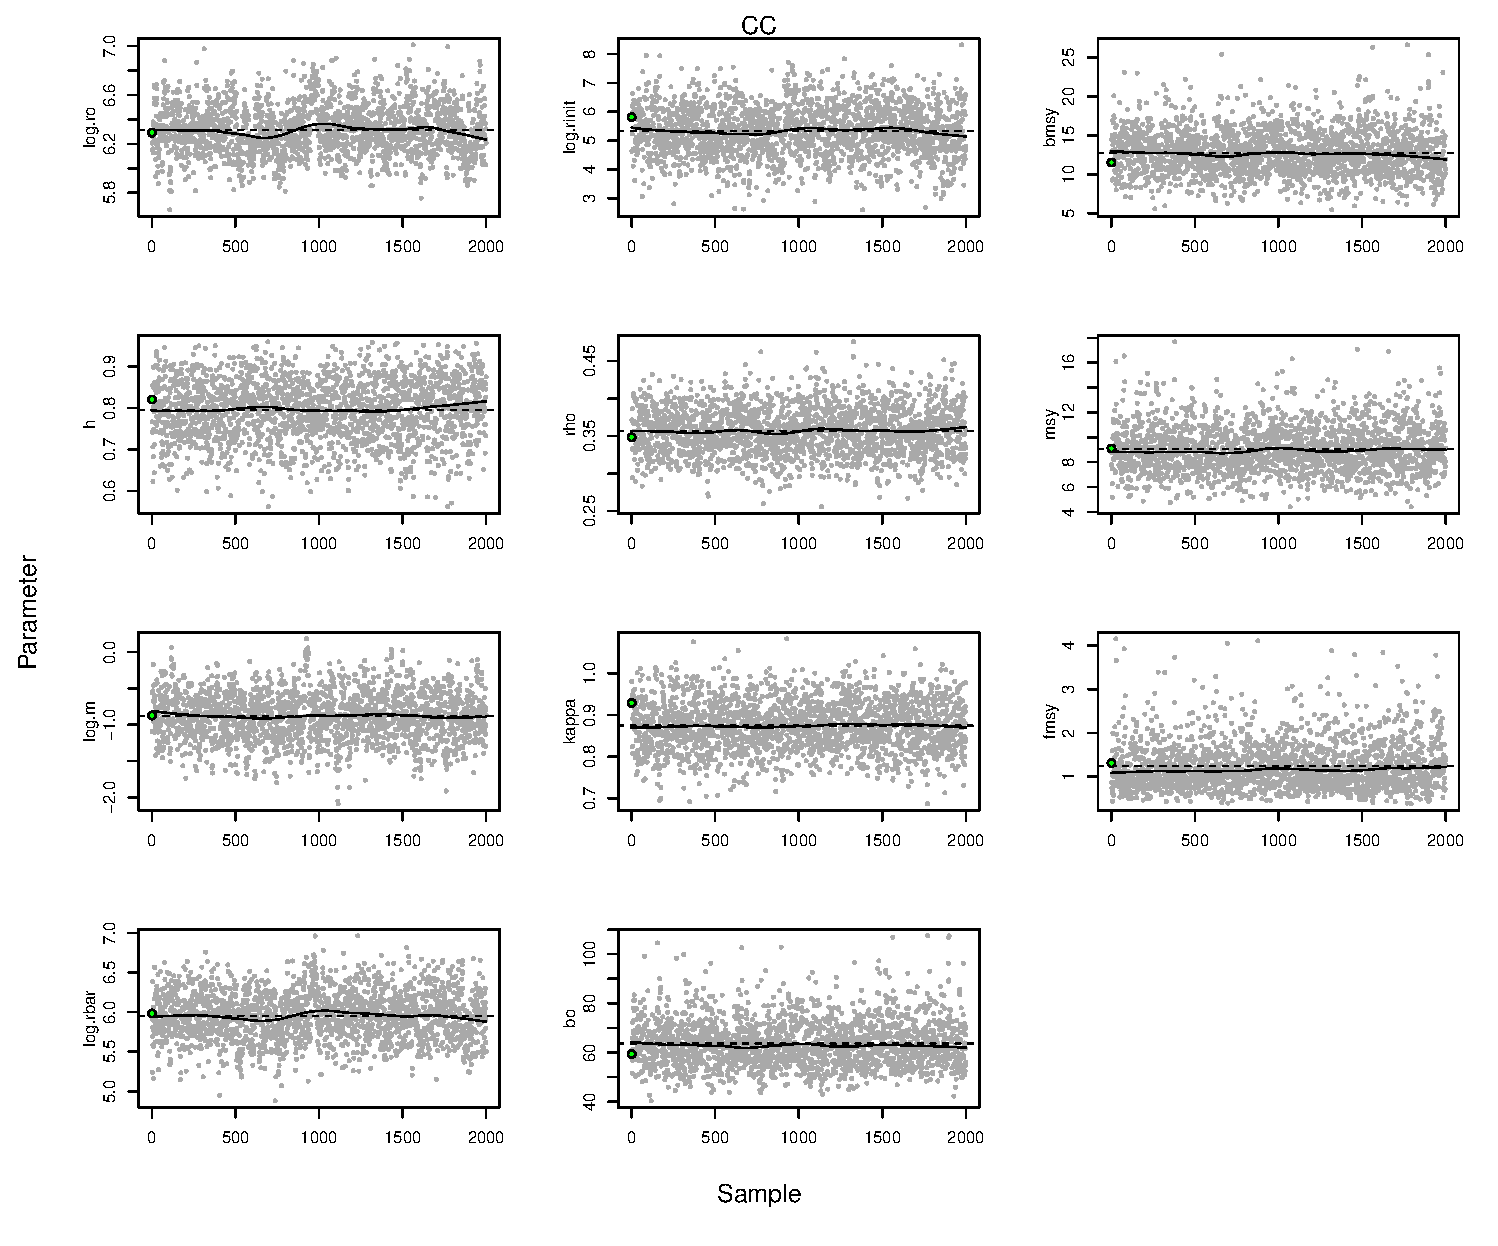
\includegraphics[width=0.9\textwidth]{../FIGS/qPriorFigs/iscam_fig_trace_CC.pdf}\\
	\caption{A systematic sample of 2,000 from an MCMC chain of length 1,000,000 of leading parameters and derived variables used in reference point calculations for CC. Green circle corresponds to the MLE estimates and the solid line is a lowess smooth fit to the data (f=1/4), and the dashed line is the mean of the distribution.}\label{PartII:MCMC:traceCC}
\end{sidewaysfigure}

\begin{sidewaysfigure}[!tbp]
	% Requires \usepackage{graphicx}
	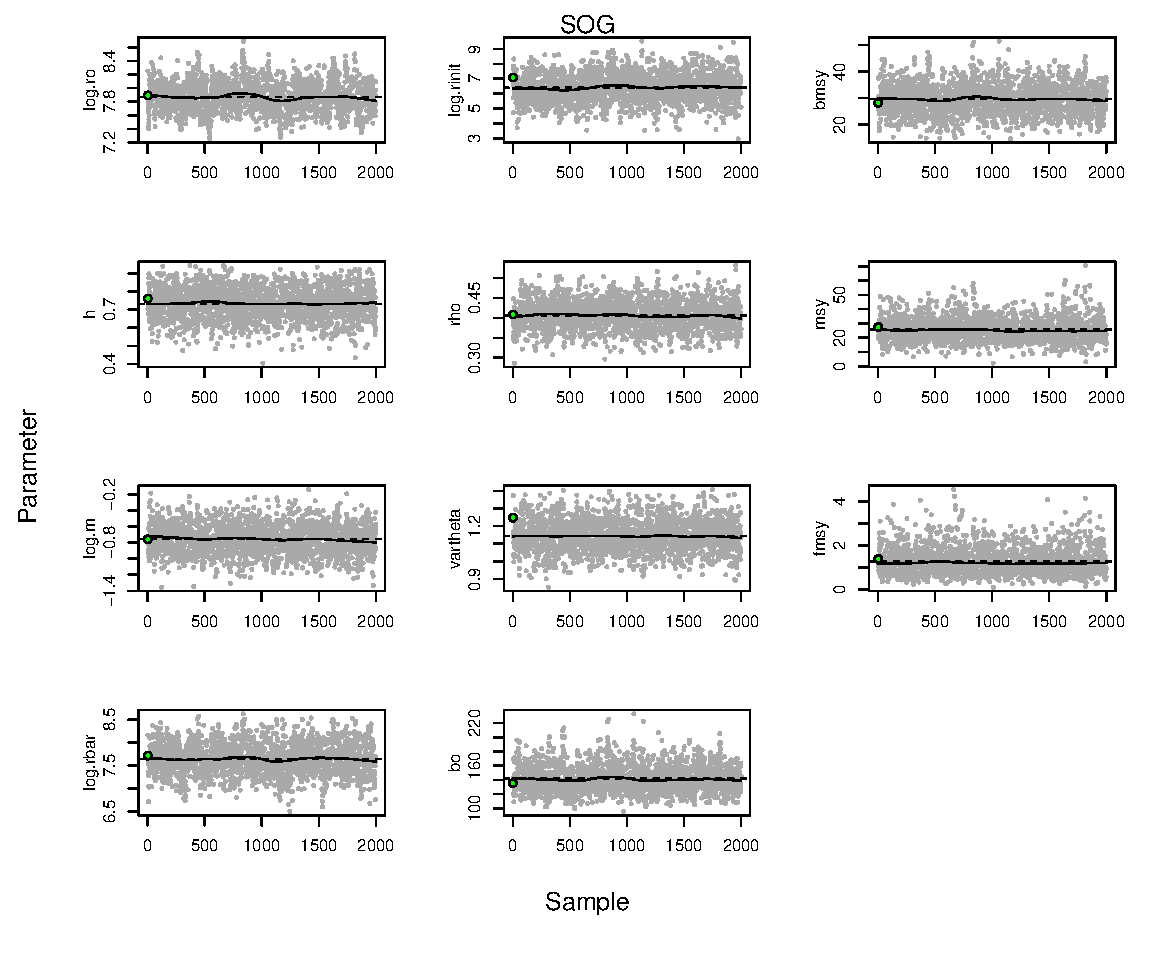
\includegraphics[width=0.9\textwidth]{../FIGS/qPriorFigs/iscam_fig_trace_SOG.pdf}\\
	\caption{A systematic sample of 2,000 from an MCMC chain of length 1,000,000 of leading parameters and derived variables used in reference point calculations for SOG. Green circle corresponds to the MLE estimates and the solid line is a lowess smooth fit to the data (f=1/4), and the dashed line is the mean of the distribution.}\label{PartII:MCMC:traceSOG}
\end{sidewaysfigure}

\begin{sidewaysfigure}[!tbp]
	% Requires \usepackage{graphicx}
	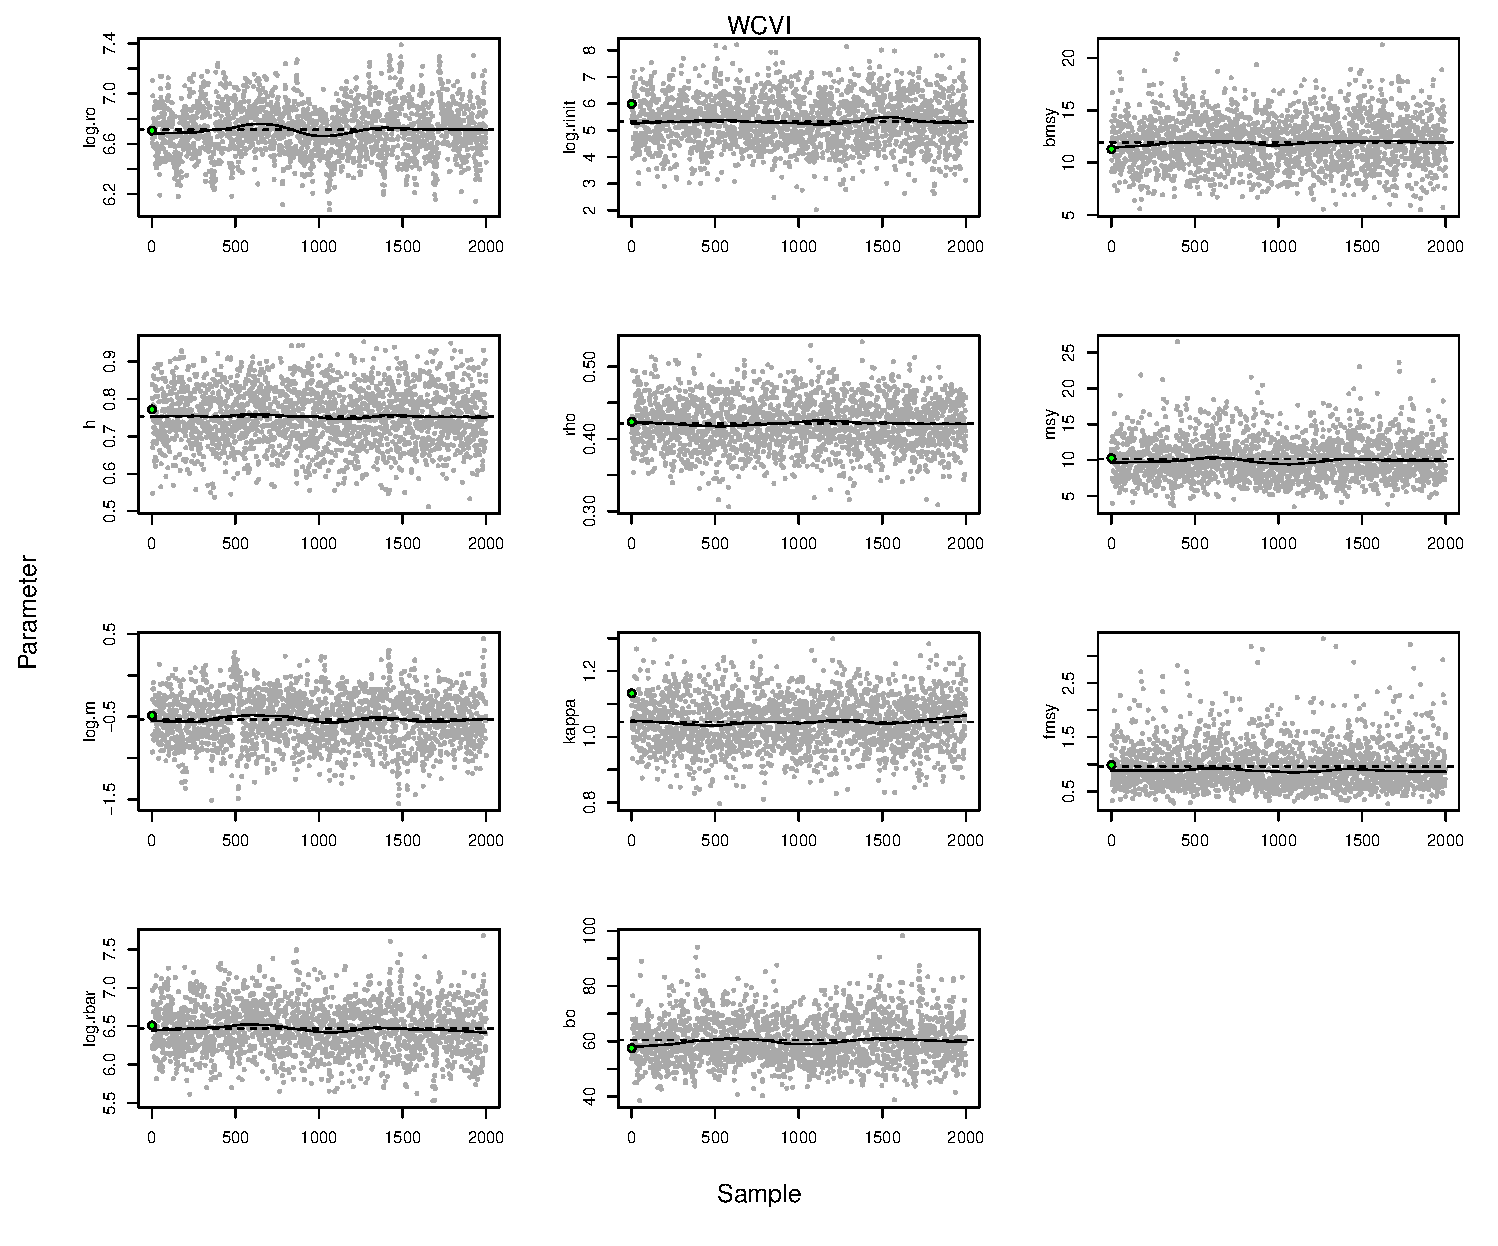
\includegraphics[width=0.9\textwidth]{../FIGS/qPriorFigs/iscam_fig_trace_WCVI.pdf}\\
	\caption{A systematic sample of 2,000 from an MCMC chain of length 1,000,000 of leading parameters and derived variables used in reference point calculations for WCVI. Green circle corresponds to the MLE estimates and the solid line is a lowess smooth fit to the data (f=1/4), and the dashed line is the mean of the distribution.}\label{PartII:MCMC:traceWCVI}
\end{sidewaysfigure}


\subsection{Parameter confounding}

To examine the level of confounding among the estimated parameters, 200 randomly selected points from the joint posterior distribution for the seven leading parameters were plotted against each other in a pairs plot (e.g., Fig. \ref{PartII:MCMC:pairsHG}). Only 200 points were plotted to reduce the file size.   Among the seven leading estimated parameters ($R_0,h,M,\bar{R},\ddot{R}, \rho, \vartheta$) there was very little confounding (Figures \ref{PartII:MCMC:pairsHG} -- \ref{PartII:MCMC:pairsWCVI}).

There is, however, some strong confounding between the estimated parameters and a few of the derived reference points.  In all major areas, there was a strong positive correlation between steepness ($h$) and \fmsy; similarly there is a strong positive correlation between \bo and $R_0$.  Among the reference points alone, there is a negative correlation between \bmsy and \fmsy, and a positive correlation between \fmsy and MSY.  This level of confounding among the derived variables is not cause for concern  from a parameter estimation standpoint; it does, however,  highlight the tradeoffs that must be made from a decision makers perspective.


\begin{figure}[!tbp]
	% Requires \usepackage{graphicx}
	\includegraphics[width=\textwidth]{../FIGS/qPriorFigs/iscam_fig_pairs_HG.pdf}\\
	\caption{Pairs plot and marginal distributions for leading parameters in HG region (200 random samples).  The dotted lines correspond to the means of the distributions, circle is the mean, and the red square is the mode of the distribution.}\label{PartII:MCMC:pairsHG}
\end{figure}


\begin{figure}[!tbp]
	% Requires \usepackage{graphicx}
	\includegraphics[width=\textwidth]{../FIGS/qPriorFigs/iscam_fig_pairs_PRD.pdf}\\
	\caption{Pairs plot and marginal distributions for leading parameters in PRD region (200 random samples).  The dotted lines correspond to the means of the distributions, circle is the mean, and the red square is the mode of the distribution.}\label{PartII:MCMC:pairsPRD}
\end{figure}

\begin{figure}[!tbp]
	% Requires \usepackage{graphicx}
	\includegraphics[width=\textwidth]{../FIGS/qPriorFigs/iscam_fig_pairs_CC.pdf}\\
	\caption{Pairs plot and marginal distributions for leading parameters in CC region (200 random samples).  The dotted lines correspond to the means of the distributions, circle is the mean, and the red square is the mode of the distribution.}\label{PartII:MCMC:pairsCC}
\end{figure}

\begin{figure}[!tbp]
	% Requires \usepackage{graphicx}
	\includegraphics[width=\textwidth]{../FIGS/qPriorFigs/iscam_fig_pairs_SOG.pdf}\\
	\caption{Pairs plot and marginal distributions for leading parameters in SOG region (200 random samples).  The dotted lines correspond to the means of the distributions, circle is the mean, and the red square is the mode of the distribution.}\label{PartII:MCMC:pairsSOG}
\end{figure}

\begin{figure}[!tbp]
	% Requires \usepackage{graphicx}
	\includegraphics[width=\textwidth]{../FIGS/qPriorFigs/iscam_fig_pairs_WCVI.pdf}\\
	\caption{Pairs plot and marginal distributions for leading parameters in WCVI region (200 random samples).  The dotted lines correspond to the means of the distributions, circle is the mean, and the red square is the mode of the distribution.}\label{PartII:MCMC:pairsWCVI}
\end{figure}

%%%%%%%%%%%%%%%%%%%%%%%%%%%%%%%%%%%%%%%%%%%%%%%%%%%%%%%%%%%%%%%
%%%%%%%%%%%%%%%%%%%%%%%%%%%%%%%%%%%%%%%%%%%%%%%%%%%%%%%%%%%%%%%
\subsection{Marginal posterior distributions}

Marginal posterior distributions and along with the prior densities for the seven leading parameters are shown in Figure \ref{PartII:MCMC:Marginals}. In all cases, the steepness parameter, followed by the instantaneous natural mortality rate appears to be the most influenced by the prior density. Uniform prior distributions were assumed for the scaling parameters ($R_0, \bar{R}$, and $\ddot{R}$).  There were good posterior updates for the total variance and variance portioning parameters ($\vartheta, \rho$).

\begin{figure}[!tbp]
	% Requires \usepackage{graphicx}
	\centering
	\setlength\fboxsep{0pt}
\setlength\fboxrule{0.5pt}
%\fbox{\includegraphics{chick}}
	\fbox{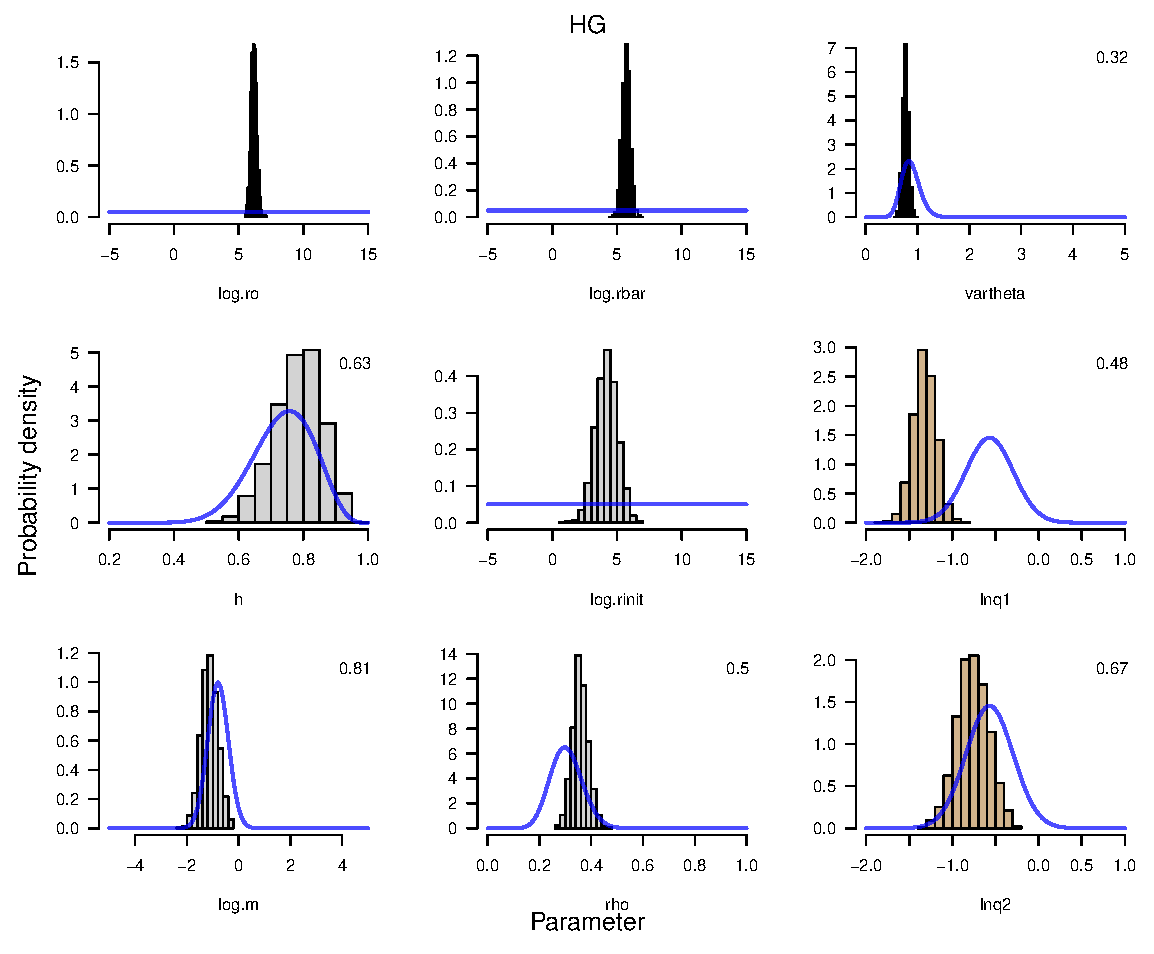
\includegraphics[width=0.49\textwidth]{../FIGS/qPriorFigs/iscam_fig_marginals_HG.pdf}}
	\fbox{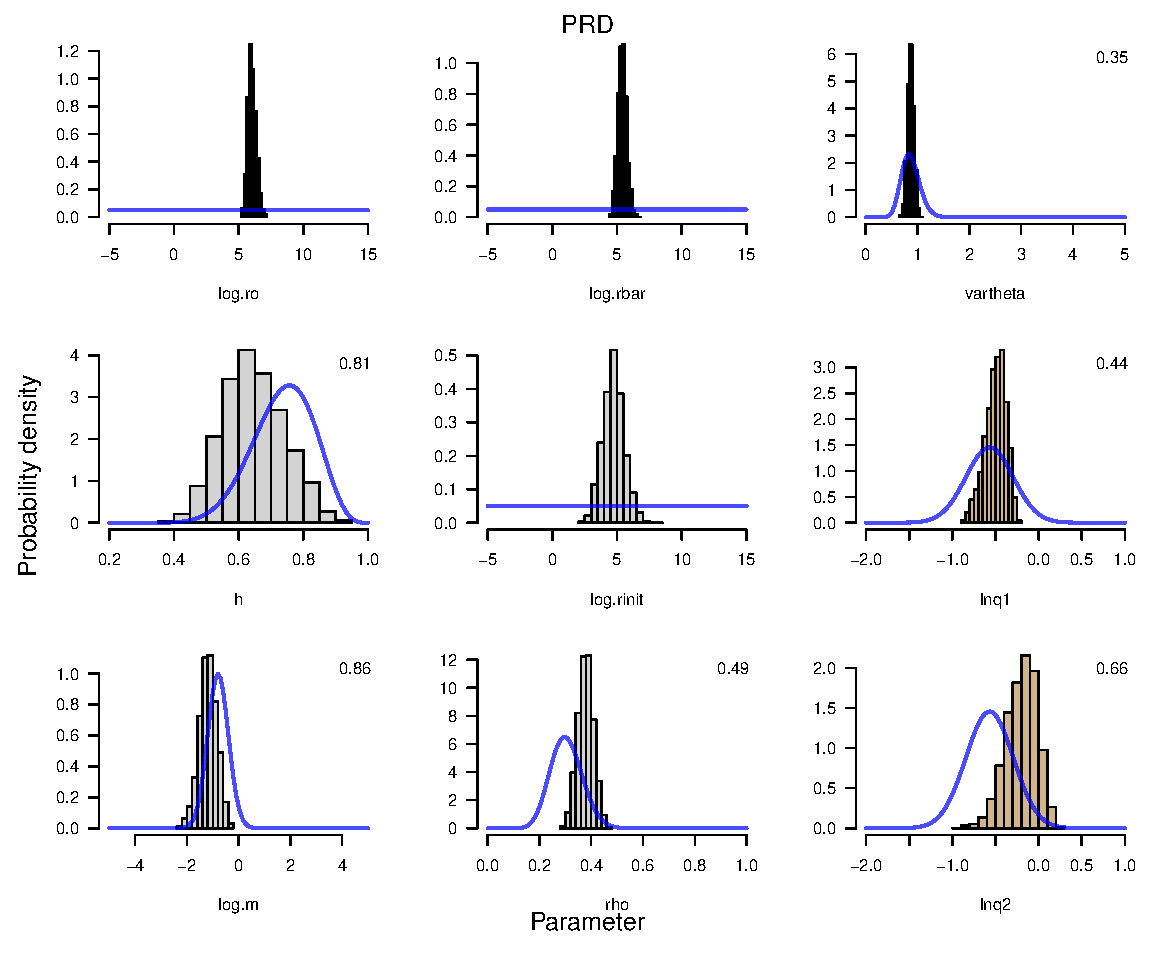
\includegraphics[width=0.49\textwidth]{../FIGS/qPriorFigs/iscam_fig_marginals_PRD.pdf}}
	\fbox{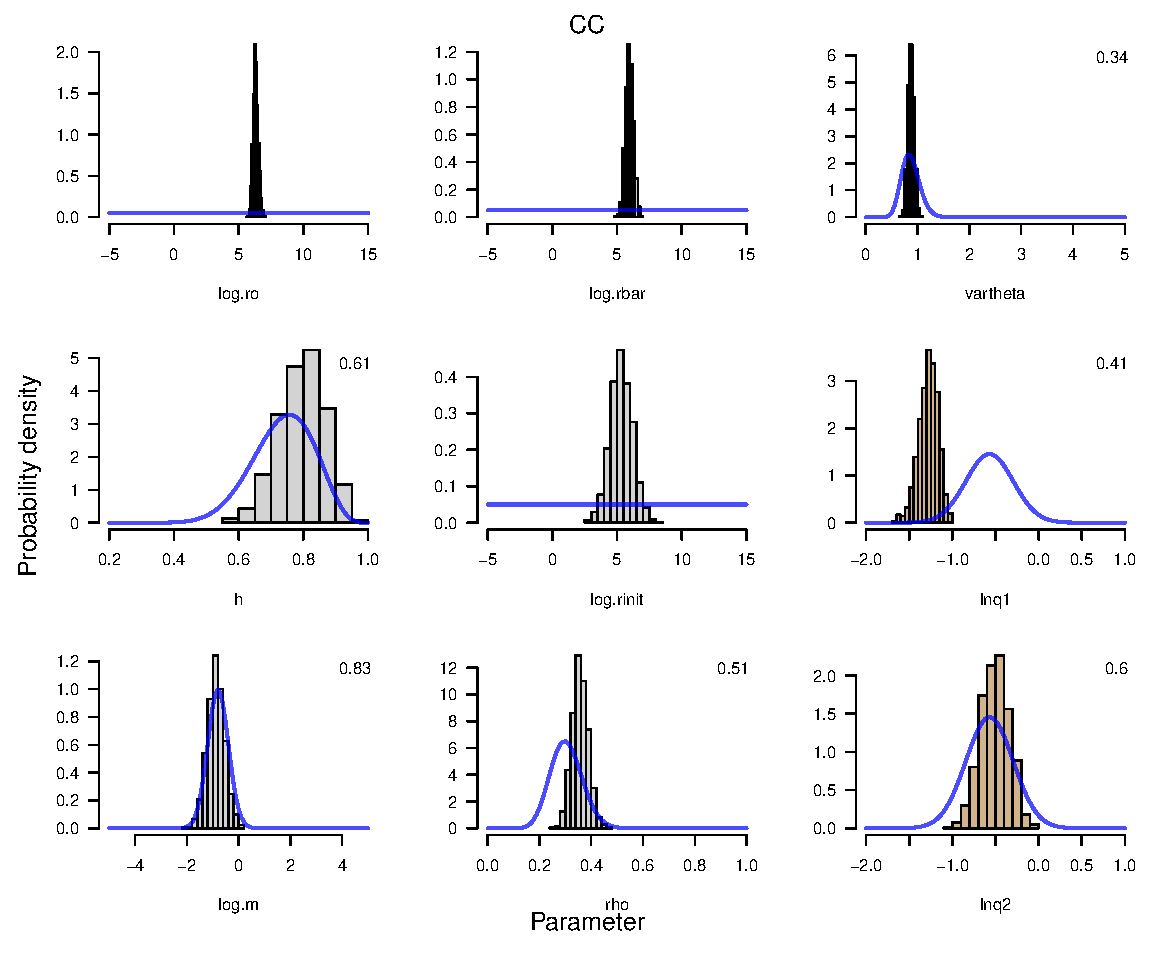
\includegraphics[width=0.49\textwidth]{../FIGS/qPriorFigs/iscam_fig_marginals_CC.pdf}}
	\fbox{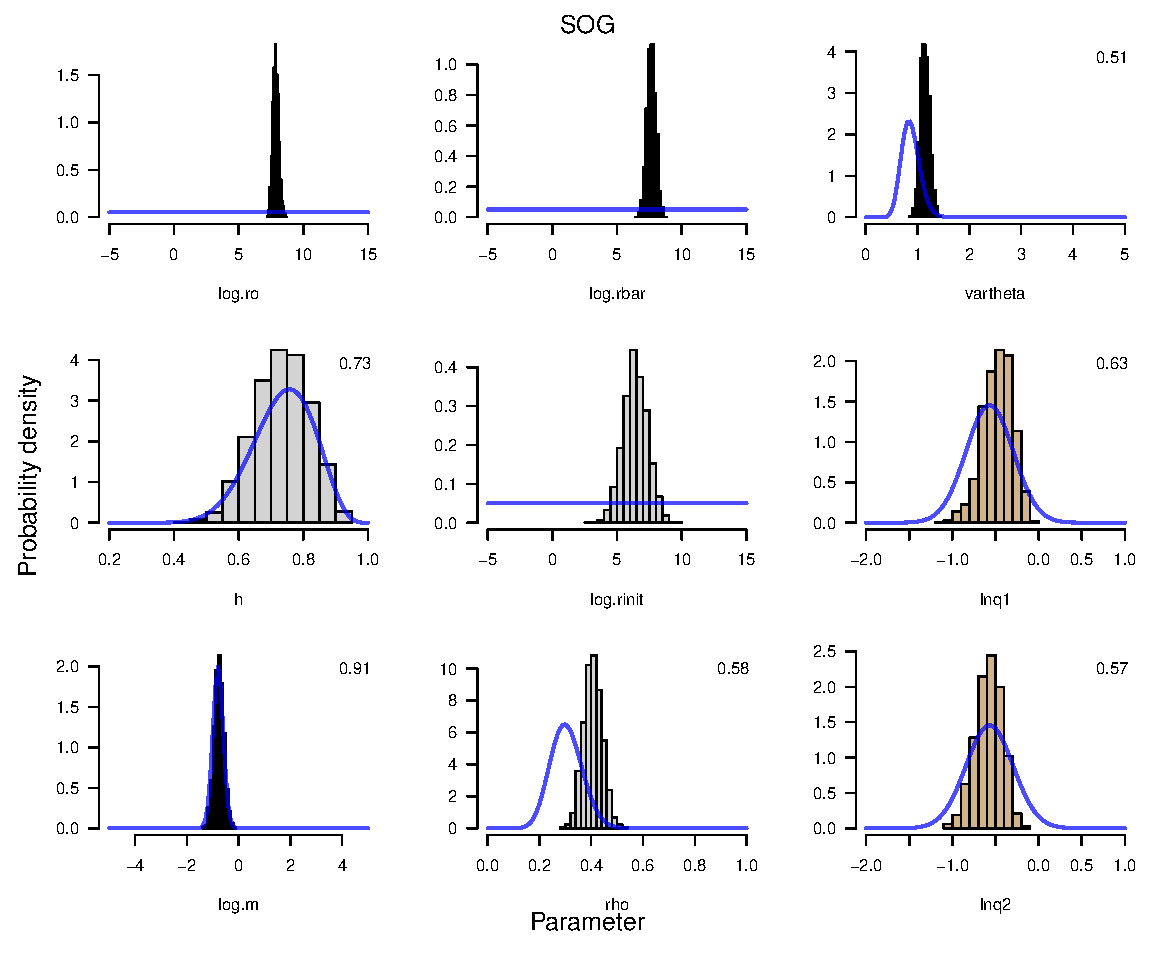
\includegraphics[width=0.49\textwidth]{../FIGS/qPriorFigs/iscam_fig_marginals_SOG.pdf}}
	\fbox{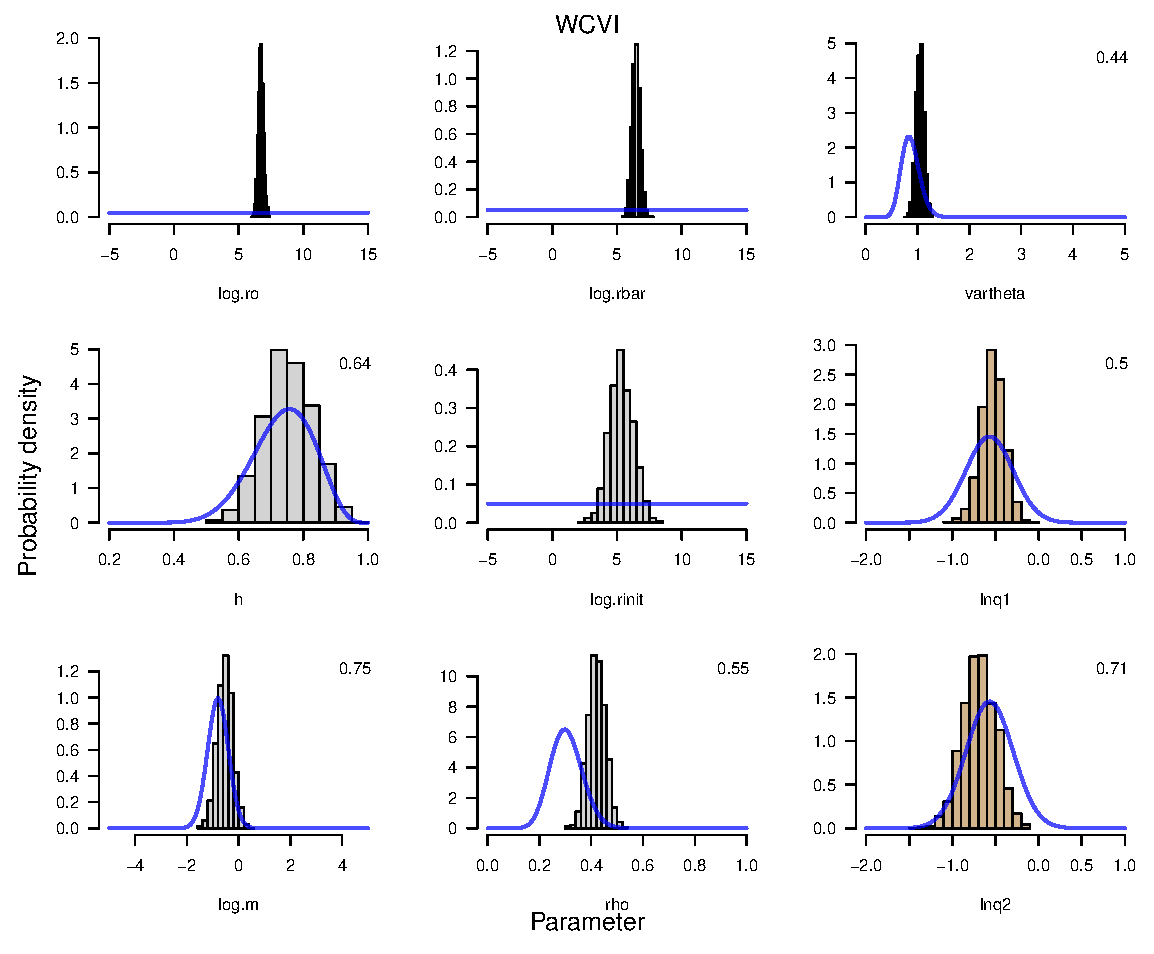
\includegraphics[width=0.49\textwidth]{../FIGS/qPriorFigs/iscam_fig_marginals_WCVI.pdf}}

	\caption{Marginal posterior densities (histograms) and prior densities (lines) for the seven leading parameters and spawn survey scaler ($\ln(q)$, tan colour) for each of the five major assessment regions.}\label{PartII:MCMC:Marginals}
\end{figure}

Median estimates of the 2011 spawning stock biomass and the 95\% credible interval for each of the five major assessment regions are summarized in Table \ref{table:2011_SB_Depletion}.  Current estimates of depletion and the corresponding uncertainty is based on the ratio of the 2011 spawning biomass divided by the corresponding estimate of \bo.  Depletion levels less that 0.25 would be considered to be below the cutoff level.

\begin{table}
	\caption{Estimates of 2011 spawning biomass, $B_0$, and depletion based on 2000 systematic samples from the joint posterior distribution drawn from a chain of length 1,000,000.\label{table:2011_SB_Depletion}}
	\begin{center}
	\begin{small}
	\begin{tabular}{l>{\bfseries}ccc|>{\bfseries}ccc|>{\bfseries}ccc}
	\hline 
	&\multicolumn{3}{c}{$SB_{2011}$} 
	&\multicolumn{3}{c}{$B_0$} 
	&\multicolumn{3}{c}{$SB_{2011}/B_0$}\\
	Stock 
	&Median & 2.5\% & 97.5\%
	&Median & 2.5\% & 97.5\%
	&Median & 2.5\% & 97.5\% \\
	\hline
	HG & 16.58 & 7.70 &33.63& 41.74 &30.05 &61.51&  0.39  &0.19  &0.75 \\
	PRD & 27.05 & 14.45&  50.59 & 78.56 & 54.15 &150.18 &  0.34  & 0.15  & 0.68\\
	CC & 14.67 & 7.28 &27.28 &62.40& 48.47& 85.06 & 0.23 & 0.12 & 0.41\\
	SOG & 125.14 & 70.43& 217.95 &140.05& 110.47& 184.24 &  0.89 &  0.53 &  1.45\\
	WCVI & 14.68 & 6.99 &27.63& 59.58& 46.84& 78.53&  0.24 & 0.12&  0.43\\
	\hline
	\end{tabular}
	\end{small}
	\end{center}
\end{table}


%%%%%%%%%%%%%%%%%%%%%%%%%%%%%%%%%%%%%%%%%%%%%%%%%%%%%%%%%%%%%%%
%%%%%%%%%%%%%%%%%%%%%%%%%%%%%%%%%%%%%%%%%%%%%%%%%%%%%%%%%%%%%%%

\subsection{Forecast and catch advice based on the joint posterior distribtution} \label{Section:Forecast}

Catch advice has historically been provided in the form of a decision table based on median values of the joint posterior distribution.  The decision table contains columns specifying the 2011 SSB the age 4+ total biomass, estimates of age-3 recruit biomass for poor, average, and good recruitment, cutoff levels, and the available harvest under poor, average, and good recruitment scenarios.  Moving towards DFO's sustainable fisheries framework  (SFF) is a necessary next step.

Cutoff levels for the BC herring stocks is defined as 0.25\bo. The historical cutoff levels have not been updated for over 10 years now (1996/1997).  Recent stock assessments (since 2001) for BC herring have assumed $q=1$ for the spawn survey data.  In this assessment we have relaxed this assumption and as a consequence estimates of herring biomass have increased substantially.  Due to significant changes in population scaling it would not make sense to continue to use the previous cutoff levels as this may lead to policies that would result in overfishing or under utilization of the resource.  We therefore present catch advice based on both the old cutoffs and the new cutoffs in Tables \ref{TableCatchAdviceOldCuttoffs}-\ref{TableCatchAdviceNewCuttoffs} 


% latex.default(xTable, file = fn, rowname = NULL, longtable = FALSE,      landscape = FALSE, cgroup = cgrp, n.cgroup = ncgrp, caption = cap,      label = "TableCatchAdvice", na.blank = TRUE, vbar = FALSE,      size = "small") 
%
\begin{table}[!tbp]
 \small
 \caption{Estimated spawning stock biomass,  age-4+ biomass and pre-fishery
			biomass for poor average and good recruitment, old cutoffs,  and 
			available harvest based on median values from the joint posterior distribution.\label{TableCatchAdviceOldCuttoffs}} 
 \begin{center}
 \begin{tabular}{lllclllclclll}\hline\hline
\multicolumn{3}{c}{\bfseries }&
\multicolumn{1}{c}{\bfseries }&
\multicolumn{3}{c}{\bfseries Pre-fishery forecast biomass}&
\multicolumn{1}{c}{\bfseries }&
\multicolumn{1}{c}{\bfseries }&
\multicolumn{1}{c}{\bfseries }&
\multicolumn{3}{c}{\bfseries Available harvest}
\tabularnewline \cline{1-13}
\multicolumn{1}{c}{Stock}&\multicolumn{1}{c}{SSB}&\multicolumn{1}{c}{4+ Biomass}&\multicolumn{1}{c}{}&\multicolumn{1}{c}{Poor}&\multicolumn{1}{c}{Average}&\multicolumn{1}{c}{Good}&\multicolumn{1}{c}{}&\multicolumn{1}{c}{Cutoff}&\multicolumn{1}{c}{}&\multicolumn{1}{c}{Poor}&\multicolumn{1}{c}{Average}&\multicolumn{1}{c}{Good}\tabularnewline
\hline
HG&16,579& 7,089&& 9,618&12,892&21,478&&10,700&&     0& 2,192& 4,296\tabularnewline
PRD&27,046&20,593&&24,150&27,492&37,286&&12,100&& 4,830& 5,498& 7,457\tabularnewline
CC&14,666& 7,809&&11,357&14,709&22,883&&17,600&&     0&     0& 4,577\tabularnewline
SOG&125,261& 72,937&& 94,703&112,856&138,448&& 21,200&& 18,941& 22,571& 27,690\tabularnewline
WCVI&14,679& 8,267&&15,321&20,906&31,130&&18,800&&     0& 2,106& 6,226\tabularnewline
\hline
\end{tabular}

\end{center}

\end{table}


% latex.default(xTable, file = fn, rowname = NULL, longtable = FALSE,      landscape = FALSE, cgroup = cgrp, n.cgroup = ncgrp, caption = cap,      label = "TableCatchAdvice", na.blank = TRUE, vbar = FALSE,      size = "small") 
%
\begin{table}[!tbp]
 \small
 \caption{Estimated spawning stock biomass,  age-4+ biomass and pre-fishery biomass for poor average and good recruitment, new cutoffs (based on median value of 0.25\bo\ estimated within the \iscam\ model), and available harvest based on the median values from the joint posterior distribtuion.\label{TableCatchAdviceNewCuttoffs}} 
 \begin{center}
 \begin{tabular}{lllclllclclll}\hline\hline
\multicolumn{3}{c}{\bfseries }&
\multicolumn{1}{c}{\bfseries }&
\multicolumn{3}{c}{\bfseries Pre-fishery forecast biomass}&
\multicolumn{1}{c}{\bfseries }&
\multicolumn{1}{c}{\bfseries }&
\multicolumn{1}{c}{\bfseries }&
\multicolumn{3}{c}{\bfseries Available harvest}
\tabularnewline \cline{1-13}
\multicolumn{1}{c}{Stock}&\multicolumn{1}{c}{SSB}&\multicolumn{1}{c}{4+ Biomass}&\multicolumn{1}{c}{}&\multicolumn{1}{c}{Poor}&\multicolumn{1}{c}{Average}&\multicolumn{1}{c}{Good}&\multicolumn{1}{c}{}&\multicolumn{1}{c}{Cutoff}&\multicolumn{1}{c}{}&\multicolumn{1}{c}{Poor}&\multicolumn{1}{c}{Average}&\multicolumn{1}{c}{Good}\tabularnewline
\hline
HG&16,579& 7,089&& 9,618&12,892&21,478&&10,436&&     0& 2,456& 4,296\tabularnewline
PRD&27,046&20,593&&24,150&27,492&37,286&&19,641&& 4,510& 5,498& 7,457\tabularnewline
CC&14,666& 7,809&&11,357&14,709&22,883&&15,600&&     0&     0& 4,577\tabularnewline
SOG&125,261& 72,937&& 94,703&112,856&138,448&& 35,013&& 18,941& 22,571& 27,690\tabularnewline
WCVI&14,679& 8,267&&15,321&20,906&31,130&&14,894&&   427& 4,181& 6,226\tabularnewline
\hline
\end{tabular}

\end{center}

\end{table}




In addition to Tables \ref{TableCatchAdviceOldCuttoffs} and \ref{TableCatchAdviceNewCuttoffs} we also provide an additional risk-based decision table that attempts to integrate over all of the uncertainty in the model (Tables \ref{Table:RiskCC}-\ref{Table:RiskWCVI}).  This decision table is also represented graphically in Figure \ref{fig:Risk}.  Figure \ref{fig:Risk} should be interpreted as follows: the probability of the spawning stock biomass falling below the cutoff level is determined by drawing a vertical line that intersect the cumulative probability curve and reading off the corresponding probability level. The reverse of this process was used to construct Tables \ref{Table:RiskCC}-\ref{Table:RiskWCVI}.
\clearpage
% latex.default(TAC, file = fn, title = "Risk", longtable = FALSE,      landscape = FALSE, cgroup = NULL, n.cgroup = NULL, caption = cap,      label = paste("Table:Risk", hdr$Stock[i], sep = ""), na.blank = TRUE,      vbar = FALSE) 
%
\begin{table}[!tbp]
 \caption{Decision table for HG where the risk 
			level represents the probability of exceeding the quantities specified
			in the headers of each column.  Three performance measures are considered:
			the probability of the spawning stock biomass in 2013 falling below the cutoff
			level,  the probability of the spawning stock biomass in 2013 declining from 2012, 
			and the probability of 2012 exploitation rate exceeding the 20\% level that is
			used in the harvest control rule. To use this table, first determine the 
			appropriate level of risk (e.g. 0.25 or 25\% chance),  then choose the appropriate
			management quantity (e.g. spawning biomass falling below the cutoff), and then read
			off the recommended catch (e.g.,  3,060 tonnes).\label{Table:RiskHG}} 
 \begin{center}
 \begin{tabular}{llll}\hline\hline
\multicolumn{1}{c}{Risk level}&\multicolumn{1}{c}{$P(SB_{2013})\textless$Cutoff}&\multicolumn{1}{c}{$P(SB_{2013}<SB_{2012})$}&\multicolumn{1}{c}{$P(U_{2012}<0.2)$}\tabularnewline
\hline
0.05&     0&     0& 2,228\tabularnewline
0.1&     0&     0& 3,552\tabularnewline
0.15&   583&     0& 4,372\tabularnewline
0.2& 1,940&     0& 4,989\tabularnewline
0.25& 3,060&     0& 5,498\tabularnewline
0.3& 4,039&     0& 5,944\tabularnewline
0.35& 4,928&     0& 6,348\tabularnewline
0.4& 5,760&     0& 6,727\tabularnewline
0.45& 6,558&     0& 7,090\tabularnewline
0.5& 7,340&     0& 7,445\tabularnewline
0.55& 8,121&     0& 7,801\tabularnewline
0.6& 8,919&   907& 8,164\tabularnewline
0.65& 9,751& 2,547& 8,542\tabularnewline
0.7&10,640& 4,299& 8,947\tabularnewline
0.75&11,619& 6,229& 9,392\tabularnewline
0.8&12,740& 8,439& 9,902\tabularnewline
0.85&14,096&11,113&10,519\tabularnewline
0.9&15,898&14,666&11,338\tabularnewline
0.95&18,809&20,404&12,662\tabularnewline
\hline
\end{tabular}

\end{center}

\end{table}


% latex.default(TAC, file = fn, title = "Risk", longtable = FALSE,      landscape = FALSE, cgroup = NULL, n.cgroup = NULL, caption = cap,      label = paste("Table:Risk", hdr$Stock[i], sep = ""), na.blank = TRUE,      vbar = FALSE) 
%
\begin{table}[!tbp]
 \caption{Decision table for PRD where the risk 
			level represents the probability of exceeding the quantities specified
			in the headers of each column.  Three performance measures are considered:
			the probability of the spawning stock biomass in 2013 falling below the cutoff
			level,  the probability of the spawning stock biomass in 2013 declining from 2012, 
			and the probability of 2012 exploitation rate exceeding the 20\% level that is
			used in the harvest control rule. To use this table, first determine the 
			appropriate level of risk (e.g. 0.25 or 25\% chance),  then choose the appropriate
			management quantity (e.g. spawning biomass falling below the cutoff), and then read
			off the recommended catch (e.g.,  1,788 tonnes).\label{Table:RiskPRD}} 
 \begin{center}
 \begin{tabular}{llll}\hline\hline
\multicolumn{1}{c}{Risk level}&\multicolumn{1}{c}{$P(SB_{2013})\textless$Cutoff}&\multicolumn{1}{c}{$P(SB_{2013}<SB_{2012})$}&\multicolumn{1}{c}{$P(U_{2012}<0.2)$}\tabularnewline
\hline
0.05&     0&    0& 3,743\tabularnewline
0.1&     0&    0& 4,914\tabularnewline
0.15&     0&    0& 5,639\tabularnewline
0.2&   655&  182& 6,185\tabularnewline
0.25& 1,788&  787& 6,636\tabularnewline
0.3& 2,777&1,315& 7,030\tabularnewline
0.35& 3,675&1,795& 7,388\tabularnewline
0.4& 4,516&2,244& 7,722\tabularnewline
0.45& 5,322&2,675& 8,043\tabularnewline
0.5& 6,112&3,097& 8,358\tabularnewline
0.55& 6,902&3,518& 8,673\tabularnewline
0.6& 7,708&3,949& 8,994\tabularnewline
0.65& 8,549&4,398& 9,328\tabularnewline
0.7& 9,447&4,878& 9,686\tabularnewline
0.75&10,437&5,406&10,080\tabularnewline
0.8&11,569&6,011&10,531\tabularnewline
0.85&12,940&6,743&11,077\tabularnewline
0.9&14,761&7,716&11,802\tabularnewline
0.95&17,702&9,287&12,973\tabularnewline
\hline
\end{tabular}

\end{center}

\end{table}


% latex.default(TAC, file = fn, title = "Risk", longtable = FALSE,      landscape = FALSE, cgroup = NULL, n.cgroup = NULL, caption = cap,      label = paste("Table:Risk", hdr$Stock[i], sep = ""), na.blank = TRUE,      vbar = FALSE) 
%
\begin{table}[!tbp]
 \caption{Decision table for CC where the risk 
			level represents the probability of exceeding the quantities specified
			in the headers of each column.  Three performance measures are considered:
			the probability of the spawning stock biomass in 2013 falling below the cutoff
			level,  the probability of the spawning stock biomass in 2013 declining from 2012, 
			and the probability of 2012 exploitation rate exceeding the 20\% level that is
			used in the harvest control rule. To use this table, first determine the 
			appropriate level of risk (e.g. 0.25 or 25\% chance),  then choose the appropriate
			management quantity (e.g. spawning biomass falling below the cutoff), and then read
			off the recommended catch (e.g.,   402 tonnes).\label{Table:RiskCC}} 
 \begin{center}
 \begin{tabular}{llll}\hline\hline
\multicolumn{1}{c}{Risk level}&\multicolumn{1}{c}{$P(SB_{2013})\textless$Cutoff}&\multicolumn{1}{c}{$P(SB_{2013}<SB_{2012})$}&\multicolumn{1}{c}{$P(U_{2012}<0.2)$}\tabularnewline
\hline
0.05&    0&     0&2,450\tabularnewline
0.1&    0& 1,521&3,195\tabularnewline
0.15&    0& 4,063&3,657\tabularnewline
0.2&    0& 5,977&4,005\tabularnewline
0.25&  402& 7,557&4,292\tabularnewline
0.3&  994& 8,938&4,543\tabularnewline
0.35&1,530&10,192&4,770\tabularnewline
0.4&2,033&11,366&4,984\tabularnewline
0.45&2,515&12,491&5,188\tabularnewline
0.5&2,987&13,593&5,388\tabularnewline
0.55&3,459&14,696&5,589\tabularnewline
0.6&3,940&15,821&5,793\tabularnewline
0.65&4,443&16,995&6,006\tabularnewline
0.7&4,980&18,249&6,234\tabularnewline
0.75&5,571&19,629&6,485\tabularnewline
0.8&6,247&21,210&6,772\tabularnewline
0.85&7,067&23,124&7,119\tabularnewline
0.9&8,155&25,665&7,581\tabularnewline
0.95&9,913&29,771&8,327\tabularnewline
\hline
\end{tabular}

\end{center}

\end{table}


% latex.default(TAC, file = fn, title = "Risk", longtable = FALSE,      landscape = FALSE, cgroup = NULL, n.cgroup = NULL, caption = cap,      label = paste("Table:Risk", hdr$Stock[i], sep = ""), na.blank = TRUE,      vbar = FALSE) 
%
\begin{table}[!tbp]
 \caption{Decision table for SOG where the risk 
			level represents the probability of exceeding the quantities specified
			in the headers of each column.  Three performance measures are considered:
			the probability of the spawning stock biomass in 2013 falling below the cutoff
			level,  the probability of the spawning stock biomass in 2013 declining from 2012, 
			and the probability of 2012 exploitation rate exceeding the 20\% level that is
			used in the harvest control rule. To use this table, first determine the 
			appropriate level of risk (e.g. 0.25 or 25\% chance),  then choose the appropriate
			management quantity (e.g. spawning biomass falling below the cutoff), and then read
			off the recommended catch (e.g., 51,565 tonnes).\label{Table:RiskSOG}} 
 \begin{center}
 \begin{tabular}{llll}\hline\hline
\multicolumn{1}{c}{Risk level}&\multicolumn{1}{c}{$P(SB_{2013})\textless$Cutoff}&\multicolumn{1}{c}{$P(SB_{2013}<SB_{2012})$}&\multicolumn{1}{c}{$P(U_{2012}<0.2)$}\tabularnewline
\hline
0.05&32,082&    0&32,080\tabularnewline
0.1&39,969&    0&37,840\tabularnewline
0.15&44,852&    0&41,406\tabularnewline
0.2&48,528&    0&44,091\tabularnewline
0.25&51,565&    0&46,308\tabularnewline
0.3&54,218&    0&48,246\tabularnewline
0.35&56,627&    0&50,005\tabularnewline
0.4&58,882&    0&51,651\tabularnewline
0.45&61,043&    0&53,230\tabularnewline
0.5&63,161&    0&54,777\tabularnewline
0.55&65,280&    0&56,324\tabularnewline
0.6&67,441&    0&57,902\tabularnewline
0.65&69,696&    0&59,549\tabularnewline
0.7&72,105&    0&61,308\tabularnewline
0.75&74,758&    0&63,245\tabularnewline
0.8&77,794&    0&65,463\tabularnewline
0.85&81,471&    0&68,148\tabularnewline
0.9&86,354&    0&71,714\tabularnewline
0.95&94,241&8,031&77,474\tabularnewline
\hline
\end{tabular}

\end{center}

\end{table}


% latex.default(TAC, file = fn, title = "Risk", longtable = FALSE,      landscape = FALSE, cgroup = NULL, n.cgroup = NULL, caption = cap,      label = paste("Table:Risk", hdr$Stock[i], sep = ""), na.blank = TRUE,      vbar = FALSE) 
%
\begin{table}[!tbp]
 \caption{Decision table for WCVI where the risk 
			level represents the probability of exceeding the quantities specified
			in the headers of each column.  Three performance measures are considered:
			the probability of the spawning stock biomass in 2013 falling below the cutoff
			level,  the probability of the spawning stock biomass in 2013 declining from 2012, 
			and the probability of 2012 exploitation rate exceeding the 20\% level that is
			used in the harvest control rule. To use this table, first determine the 
			appropriate level of risk (e.g. 0.25 or 25\% chance),  then choose the appropriate
			management quantity (e.g. spawning biomass falling below the cutoff), and then read
			off the recommended catch (e.g.,    184 tonnes).\label{Table:RiskWCVI}} 
 \begin{center}
 \begin{tabular}{llll}\hline\hline
\multicolumn{1}{c}{Risk level}&\multicolumn{1}{c}{$P(SB_{2013})\textless$Cutoff}&\multicolumn{1}{c}{$P(SB_{2013}<SB_{2012})$}&\multicolumn{1}{c}{$P(U_{2012}<0.2)$}\tabularnewline
\hline
0.05&     0&   907&2,269\tabularnewline
0.1&     0& 6,355&3,125\tabularnewline
0.15&     0& 9,728&3,655\tabularnewline
0.2&     0&12,267&4,054\tabularnewline
0.25&   184&14,365&4,384\tabularnewline
0.3&   969&16,197&4,671\tabularnewline
0.35& 1,682&17,861&4,933\tabularnewline
0.4& 2,349&19,418&5,178\tabularnewline
0.45& 2,989&20,912&5,412\tabularnewline
0.5& 3,616&22,375&5,642\tabularnewline
0.55& 4,243&23,838&5,872\tabularnewline
0.6& 4,882&25,331&6,106\tabularnewline
0.65& 5,549&26,888&6,351\tabularnewline
0.7& 6,262&28,552&6,613\tabularnewline
0.75& 7,047&30,385&6,900\tabularnewline
0.8& 7,946&32,482&7,230\tabularnewline
0.85& 9,034&35,022&7,629\tabularnewline
0.9&10,478&38,395&8,159\tabularnewline
0.95&12,812&43,842&9,015\tabularnewline
\hline
\end{tabular}

\end{center}

\end{table}



\begin{sidewaysfigure}[htbp]
	\centering
		\fbox{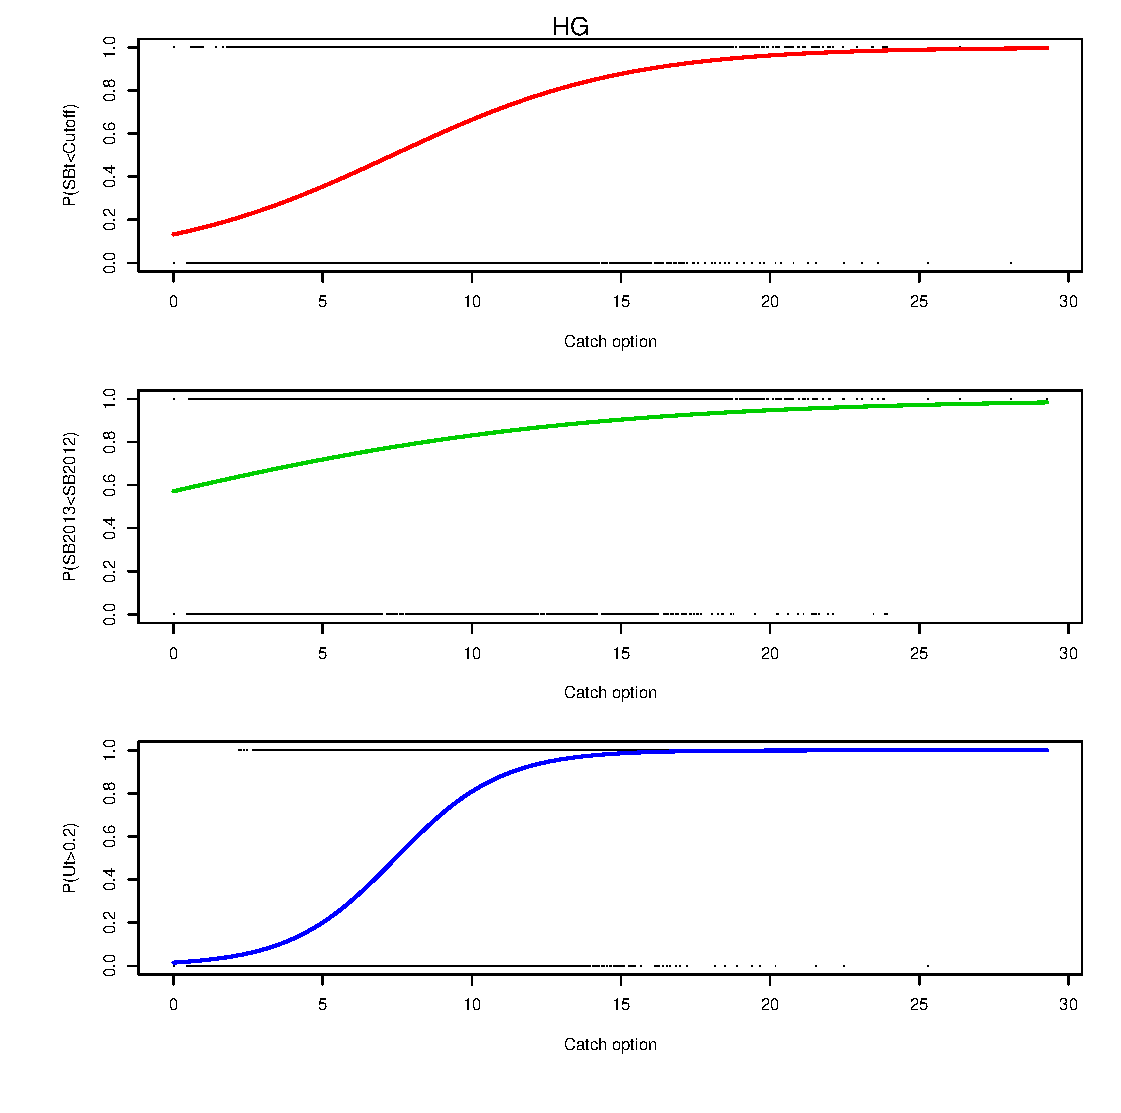
\includegraphics[width=0.32\textwidth]
		{../FIGS/qPriorFigs/iscam_fig_risk_HG}}
		\fbox{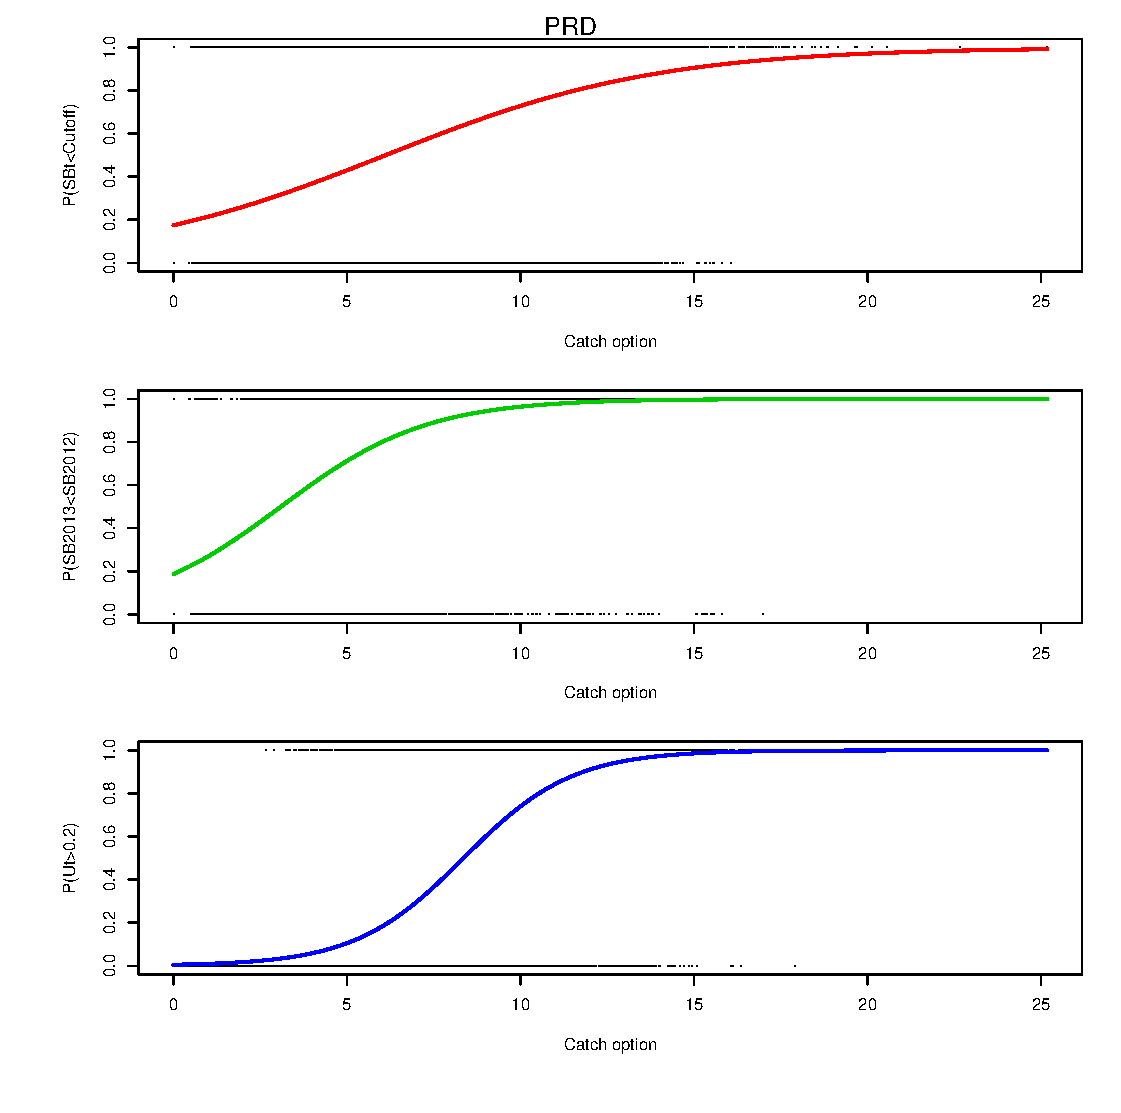
\includegraphics[width=0.32\textwidth]
		{../FIGS/qPriorFigs/iscam_fig_risk_PRD}}
		\fbox{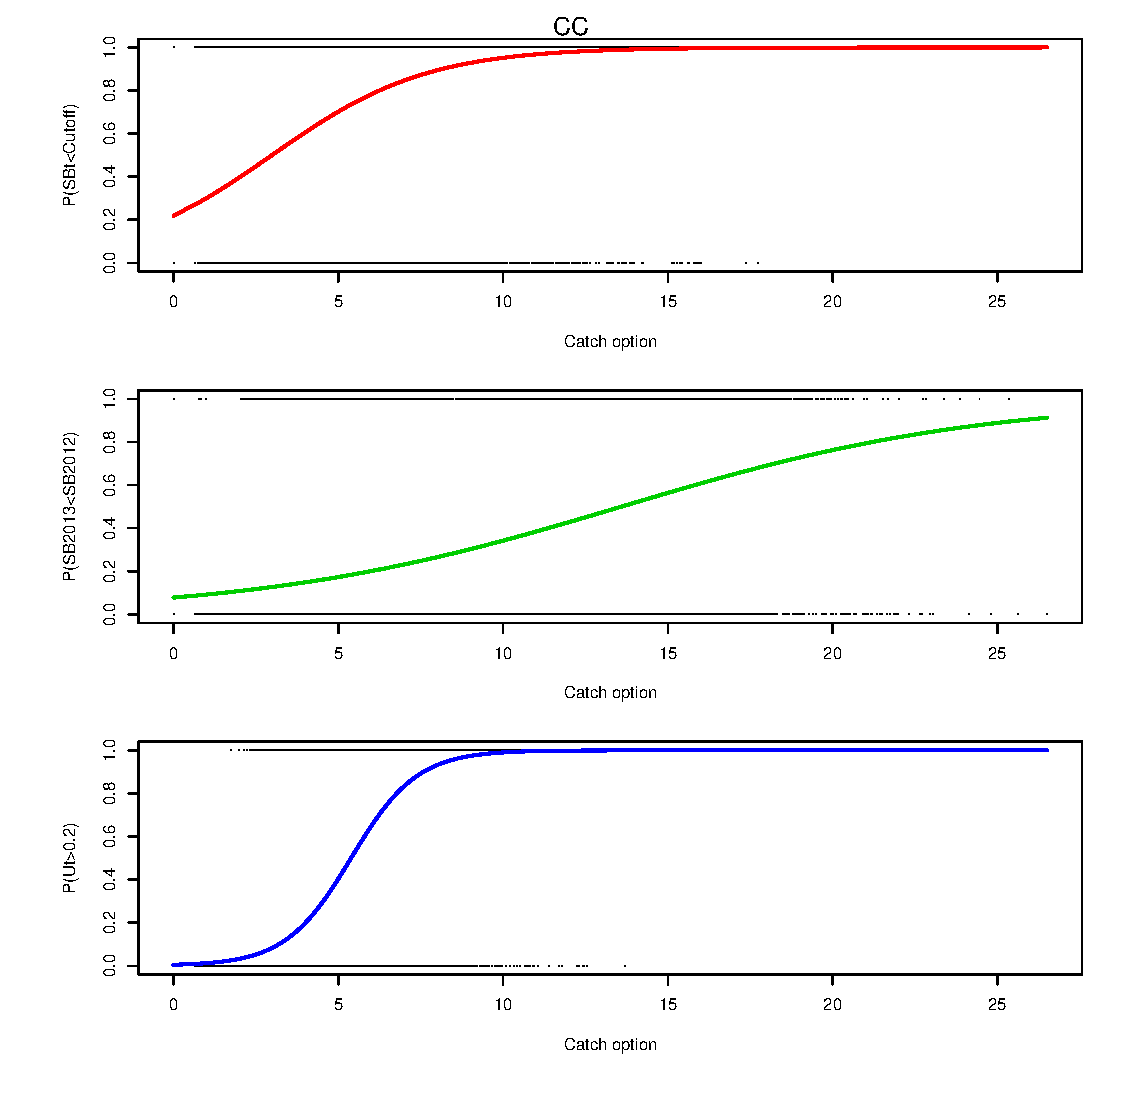
\includegraphics[width=0.32\textwidth]
		{../FIGS/qPriorFigs/iscam_fig_risk_CC}}\\
		\fbox{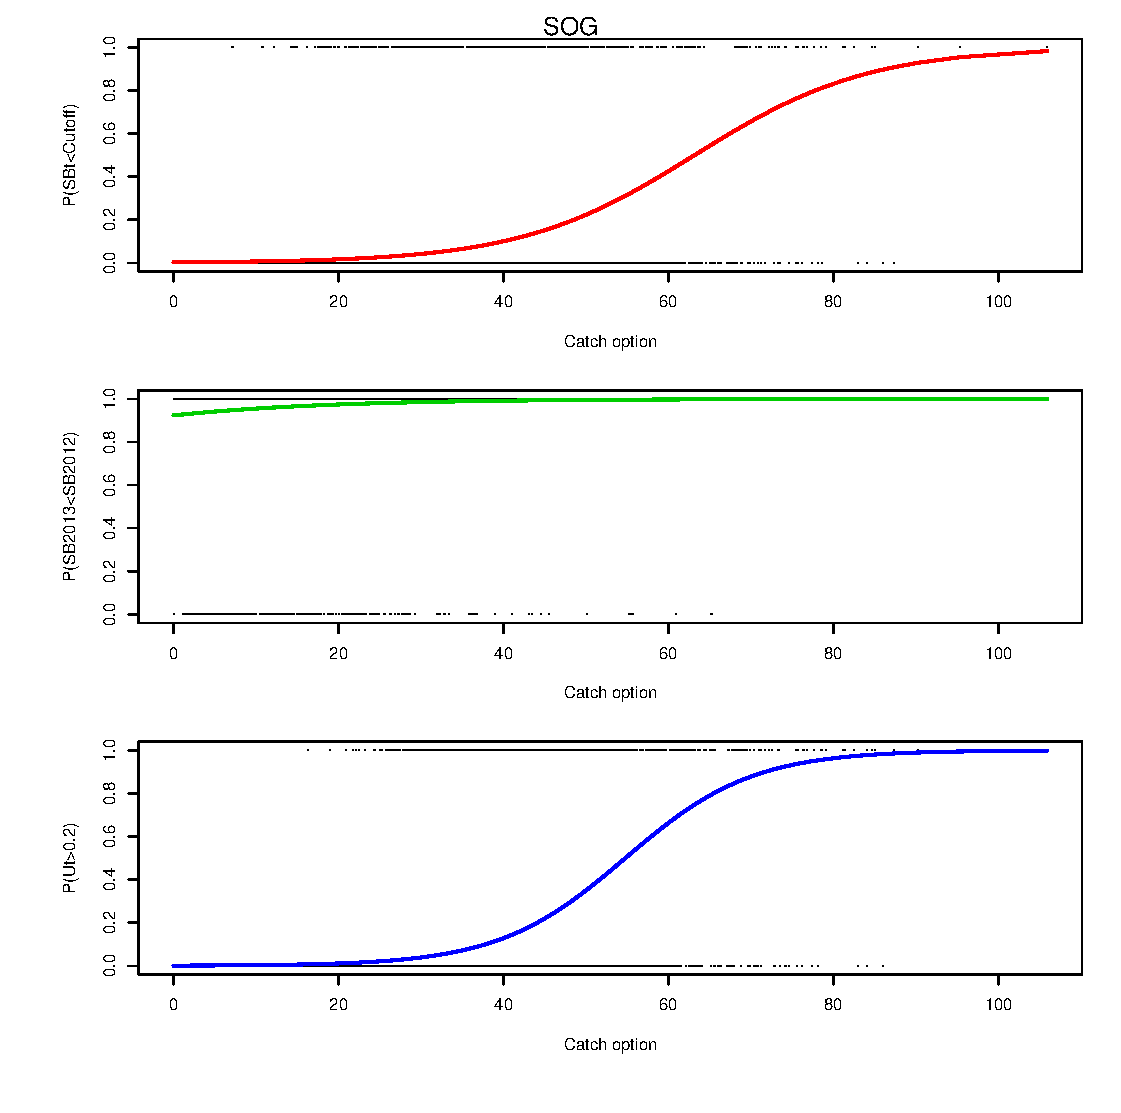
\includegraphics[width=0.32\textwidth]
		{../FIGS/qPriorFigs/iscam_fig_risk_SOG}}
		\fbox{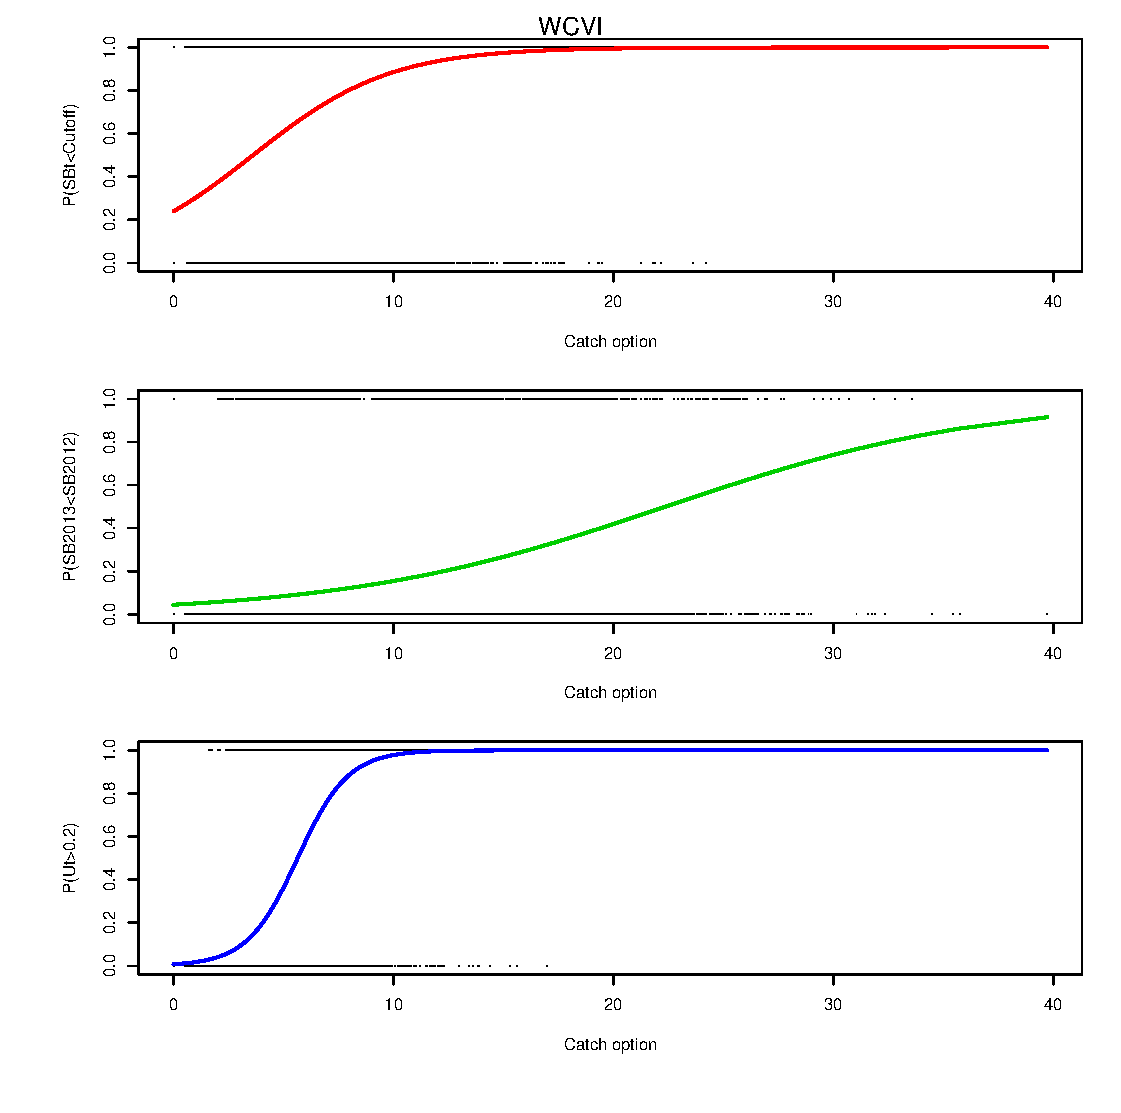
\includegraphics[width=0.32\textwidth]
		{../FIGS/qPriorFigs/iscam_fig_risk_WCVI}}
	\caption{Top Panels: probability of the spawning stock biomass in 2013 falling below the cutoff level versus the 2012 catch option. Middle Panels: probability of the spawning stock in 2013 being less than the spawning stock biomass in 2012 versus the 2012 catch option. Bottom Panels: probability of the 2012 harvest rate (catch/3+ biomass) being greater than the target harvest rate of 0.2.}
	\label{fig:Risk}
\end{sidewaysfigure}
 


%Decision table
%Notes from June Meeting:\\
%Were not completely comfortable with the q estimates, but we believe the approach used to develop the informative prior for q is better than the ad hoc q=1 assumption.  Assuming $q=1$ is more conservative as there is a tendency for $q<1$ when freely estimated with an informative prior.
